\documentclass[12pt]{article}
\usepackage{amsmath, amssymb, amsfonts, amsthm, mathtools,mathrsfs}
\usepackage{bm}
\usepackage{thmtools}
\usepackage[utf8]{inputenc}
\usepackage[inline]{enumitem}
\usepackage[colorlinks=true]{hyperref}
\usepackage{multicol}
\usepackage{witharrows}
\usepackage{tikz}
\usetikzlibrary{automata,positioning}
\usetikzlibrary{decorations.markings}
\usepackage{verbatim}
\usetikzlibrary{arrows.meta} 
\usepackage{witharrows}
\usepackage[useregional, showdow]{datetime2}
\usepackage{physics}
\DTMlangsetup[en-GB]{abbr}
\usepackage{xcolor}
\usepackage[normalem]{ulem}
\usetikzlibrary{chains,shapes.multipart}
\usepackage{algorithm}
\usepackage{algpseudocode}

\usepackage{bbm}
\usepackage[page,toc,titletoc,title]{appendix}
\usepackage{tocloft}
\setlength\parindent{0pt}
\usepackage{parskip}

\def\D{\mathrm{d}}
\def\I{\mathbb{I}}
\def\P{\mathbb{P}}
\def\E{\mathbb{E}}
\def\Var{\text{Var}}
\def\prox{\text{prox}}
\def\F{\mathcal{F}} 
\def\ccdf{\overline{F}} 
\newcommand*{\thead}[1]{\multicolumn{1}{c}{\bfseries #1}}
\renewcommand{\arraystretch}{1}
\newcommand{\indep}{\perp \!\!\! \perp}

\usepackage[framemethod=tikz]{mdframed}
\mdfdefinestyle{theoremstyle}{%
	% linecolor=gray,linewidth=1pt,%
	% frametitlerule=true,%
	frametitlebackgroundcolor=white,
	% backgroundcolor=  gray!20,	
	bottomline=false, topline=false, rightline=false, leftline=true,
	innerlinewidth=0.7pt, outerlinewidth=0.2pt, middlelinewidth=2pt, middlelinecolor=white, %
	innerleftmargin=6pt,
	% innertopmargin=-1pt,
	skipabove=10pt,
	% fontcolor=blue,
	% innerbottommargin=-0.5pt,
}
\mdtheorem[style=theoremstyle]{defn}[thm]{Definition}[section]
\mdtheorem[style=theoremstyle]{lem}[thm]{Lemma}
\mdtheorem[style=theoremstyle]{prop}[thm]{Proposition}
\mdtheorem[style=theoremstyle]{thm}{Theorem}[section]
\mdtheorem[style=theoremstyle]{cor}{Corollary}[section]


\newcommand*{\doublerule}{\hrule width \hsize height 1pt \kern 0.5mm \hrule width \hsize height 2pt}
\newcommand{\doublerulefill}{\leavevmode\leaders\vbox{\hrule width .1pt\kern1pt\hrule}\hfill\kern0pt}
\def\ddfrac#1#2{\displaystyle\frac{\displaystyle #1}{\displaystyle #2}}
\newcommand{\interior}[1]{%
  {\kern0pt#1}^{\mathrm{o}}%
}

%\newcommand{\Res}{\operatorname{Res}}

\theoremstyle{definition}
% \numberwithin{thm}{section}
% \newtheorem{lem}[thm]{Lemma}
% \newtheorem{defn}[thm]{Definition}
% \newtheorem{prop}[thm]{Proposition}
% \newtheorem{cor}[thm]{Corollary}
% \newtheorem{ex}{Example}


\let\emptyset\varnothing

\usepackage{titlesec}
\titleformat{\section}[block]{\Large\filcenter\bfseries}{\S\thesection.}{0.25cm}{\Large}
\titleformat{\subsection}[block]{\large\bfseries\sffamily}{\S\S\thesubsection.}{0.2cm}{\large}

\usepackage[a4paper]{geometry}
\usepackage{lipsum}
\usepackage{xcolor,cancel}

\usepackage{cleveref}
\crefname{thm}{Theorem}{Theorems}
\crefname{lem}{Lemma}{Lemmas}
\crefname{defn}{Definition}{Definitions}
\crefname{prop}{Proposition}{Propositions}
\crefname{cor}{Corollary}{Corollaries}
\crefname{equation}{}{}
\DeclareMathOperator*{\argmin}{argmin}
\DeclareMathOperator*{\argmax}{argmax}
\DeclareMathOperator*{\Vol}{Vol}
\DeclareMathOperator*{\co}{co}
\DeclareMathOperator*{\cco}{\overline{co}}
\DeclareMathOperator*{\diag}{diag}
\DeclareMathOperator*{\Span}{span}
\DeclareMathOperator*{\epi}{epi}

\usepackage{mdframed}
\newenvironment{blockquote}
{\begin{mdframed}[skipabove=0pt, skipbelow=0pt, innertopmargin=4pt, innerbottommargin=4pt, bottomline=false,topline=false,rightline=false, linewidth=2pt]}
{\end{mdframed}}
\newenvironment{soln}{\begin{proof}[Solution]}{\end{proof}}

\title{A First Course in Optimization\\}
\author{Ishan Kapnadak}
\date{Autumn Semester 2022-23\\~\\Updated on: \textcolor{blue}{\DTMToday}}

\begin{document}
\tikzset{lab dis/.store in=\LabDis,
  lab dis=-0.4,
  ->-/.style args={at #1 with label #2}{decoration={
    markings,
    mark=at position #1 with {\arrow{>}; \node at (0,\LabDis) {#2};}},postaction={decorate}},
  -<-/.style args={at #1 with label #2}{decoration={
    markings,
    mark=at position #1 with {\arrow{<}; \node at (0,\LabDis)
    {#2};}},postaction={decorate}},
  -*-/.style args={at #1 with label #2}{decoration={
    markings,
    mark=at position #1 with {{\fill (0,0) circle (1.5pt);} \node at (0,\LabDis)
    {#2};}},postaction={decorate}},
  }
\maketitle

\begin{abstract}
    \begin{center}
        Lecture Notes for the course EE 659: A First Course in Optimization taught in Spring 2022 by Prof. Vivek Borkar. Additional references include \textit{A first course in optimization} by Rangarajan K. Sundaram, \textit{Optimization by vector space methods} by David Luenberger, and \textit{Nonlinear programming} by Dimitri P. Bertsekas
    \end{center}
\end{abstract}

\tableofcontents
\newpage

\section{Lecture 1}
\medskip

\begin{defn}[Open Ball]
    The \emph{open ball} of radius $\epsilon$ centered around $\mathbf{x}_0 \in \mathbb{R}^d$ is defined as
    \[
        B_{\epsilon}(\mathbf{x}_0) \vcentcolon= \left\{ \mathbf{x} \in \mathbb{R}^d \colon \norm{\mathbf{x} - \mathbf{x}_0} < \epsilon \right\}.
    \]
\end{defn}
\begin{defn}[Closed Ball]
    The \emph{closed ball} of radius $\epsilon$ centered around $\mathbf{x}_0 \in \mathbb{R}^d$ is defined as
    \[
        \overline{B}_{\epsilon}(\mathbf{x}_0) \vcentcolon= \left\{ \mathbf{x} \in \mathbb{R}^d \colon \norm{\mathbf{x} - \mathbf{x}_0} \leq \epsilon \right\}.
    \]
\end{defn}
\begin{defn}[Open and Closed Sets]
    A set $A \subset \mathbb{R}^d$ is said to be \emph{open} if for all $\mathbf{x} 
    \in A$, there exists an $\epsilon > 0$ such that $B_{\epsilon}(\mathbf{x}) \subset A$. A set $A$ is said to be \emph{closed} if $A^{\mathsf{c}}$ is open.
\end{defn}

We have the following properties for open and closed sets.

\begin{enumerate}
    \item Let $\mathcal{I}$ be an arbitrary index set. If $A_{\alpha}$ is open for each $\alpha \in \mathcal{I}$, then 
    \[
        \bigcup_{\alpha \in \mathcal{I}} \, A_{\alpha}
    \]
    is open. In other words, open sets are closed under arbitrary unions.

    \item Let $\mathcal{I}$ be a finite index set. If $A_{\alpha}$ is open for each $\alpha \in \mathcal{I}$, then 
    \[
        \bigcap_{\alpha \in \mathcal{I}} \, A_{\alpha}
    \]
    is open. In other words, open sets are closed under finte intersections.

    \item Let $\mathcal{I}$ be an arbitrary index set. If $A_{\alpha}$ is closed for each $\alpha \in \mathcal{I}$, then 
    \[
        \bigcap_{\alpha \in \mathcal{I}} \, A_{\alpha}
    \]
    is closed. In other words, closed sets are closed under arbitrary intersections.

    \item Let $\mathcal{I}$ be a finite index set. If $A_{\alpha}$ is closed for each $\alpha \in \mathcal{I}$, then 
    \[
        \bigcup_{\alpha \in \mathcal{I}} \, A_{\alpha}
    \]
    is closed. In other words, closed sets are closed under finite unions.
\end{enumerate}

\begin{defn}[Convergence of a sequence]
    Let $\langle \mathbf{x}_n \rangle$ be a sequence in $\mathbb{R}^d$. Then, $\langle\mathbf{x}_n\rangle$ converges to $\mathbf{x}^*$ (written $\mathbf{x}_n \to \mathbf{x}^*$) if for all $\epsilon > 0$, there exists an $n_0 \in \mathbb{N}$ such that
    \[
        \mathbf{x}_n \in B_{\epsilon}(\mathbf{x}^*) \quad \forall n > n_0.
    \]
    Equivalently, $\norm{\mathbf{x}_n - \mathbf{x}^*} \to 0$.
\end{defn}

\begin{defn}[Closure]
    Let $A \subset \mathbb{R}^d$. The \emph{closure} of $A$ (denoted $\overline{A}$) is the smallest closed set containing $A$. Equivalently, $\overline{A}$ is the intersection of all closed sets containing $A$.
\end{defn}

\begin{defn}[Interior]
    Let $A \subset \mathbb{R}^d$. The \emph{interior} of $A$ (denoted $\interior{A}$) is the largest open set contained in $A$. Equivalently, $\interior{A}$ is the union of all open sets contained in $A$.
\end{defn}
Note that by definition, we have $\interior{A} \subset A \subset \overline{A}$.

\begin{defn}[Boundary]
    Let $A \subset \mathbb{R}^d$. The \emph{boundary} of $A$ is defined as
    \[
        \partial A \vcentcolon= \overline{A} \setminus \interior{A}.
    \]
\end{defn}
Note that for a closed set, $\overline{A} = A$, and for an open set, $\interior{A} = A$. 

\begin{prop}
    A set $A \subset \mathbb{R}^d$ is closed if and only if
    \[
        \mathbf{x}_n  \to \mathbf{x}^*, \mathbf{x}_n \in A \forall n \implies \mathbf{x}^* \in A.
    \]
\end{prop}
\begin{proof}
    Let $A \subset \mathbb{R}^d$ be closed, $\mathbf{x}_n \in A$ for all $n$, and $\mathbf{x}_n \to \mathbf{x}^*$. Assume to the contrary that $\mathbf{x}^* \notin A$. Then, $\mathbf{x}^* \in A^{\mathsf{c}}$, which is open by assumption. Thus, $\exists \epsilon > 0$ such that $B_{\epsilon}(\mathbf{x}^*) \subset A^{\mathsf{c}}$. This implies that $\mathbf{x}_n \notin B_{\epsilon}(\mathbf{x}^*)$ for all $n$, and thus $\mathbf{x}_n \not\to \mathbf{x}^*$, a contradiction. To prove the converse, assume that $A$ is not closed. Thus, there exists a $\Tilde{\mathbf{x}} \in \partial A$ such that $\Tilde{\mathbf{x}} \notin A$. Then, for all $\epsilon > 0$, $B_{\epsilon}(\Tilde{\mathbf{x}}) \cap A \neq \emptyset$. Let $\epsilon_n \downarrow 0$ and let $\mathbf{x}_n \in B_{\epsilon_n}(\Tilde{\mathbf{x}}) \cap A$. Then, $\mathbf{x}_n \to \Tilde{\mathbf{x}} \notin A$, a contradiction.
\end{proof}

\begin{defn}[Limit Point]
    Let $\langle \mathbf{x}_n \rangle$ be a sequence in $\mathbb{R}^d$. $\Tilde{\mathbf{x}}$ is a \emph{limit point} of $\langle \mathbf{x}_n \rangle$ if there exists a subsequence $\langle \mathbf{x}_{n_k} \rangle$ such that $\mathbf{x}_{n_k} \to \Tilde{\mathbf{x}}$.
\end{defn}

\begin{prop}
    $\langle \mathbf{x}_n \rangle$ converges if and only if $\langle \mathbf{x}_n \rangle$ has a unique limit point.    
\end{prop}

\begin{defn}[Supremum and Infimum]
    Let $A \subset \mathbb{R}$ be bounded. Then, 
    \begin{align*}
        \sup A &\vcentcolon= \text{ smallest } x \in \mathbb{R} \cup \{+\infty\} \text{ such that } y \in A \implies y \leq x, \\
        \inf A &\vcentcolon= \text{ largest } x \in \mathbb{R} \cup \{-\infty\} \text{ such that } y \in A \implies y \geq x.
    \end{align*}
\end{defn}

\begin{defn}[Cauchy Sequence]
    A sequence $\langle \mathbf{x}_n \rangle$ is said to be \emph{Cauchy} if $\displaystyle\lim_{m,n \uparrow \infty} \norm{\mathbf{x}_m - \mathbf{x}_n} = 0$.
\end{defn}

\begin{prop}
    Cauchy sequences are bounded.
\end{prop}
\begin{proof}
    Let $\langle \mathbf{x}_n \rangle$ be a Cauchy sequene and let $\epsilon > 0$. Pick $N$ large enough such that 
    \[
        n,m > N \implies \norm{\mathbf{x}_m - \mathbf{x}_n} < \epsilon.
    \]
    We then have
    \begin{align*}
        &\mathbf{x}_n \in B_{\epsilon}(\mathbf{x}_m) \quad \forall n > N \\
        &\implies \langle \mathbf{x}_n \colon n > N\rangle \text{ is bounded} \\
        &\implies \langle \mathbf{x}_n \rangle \text{ is bounded.} \qedhere
    \end{align*}
\end{proof} 
\begin{prop}
    Cauchy sequences have at most one limit point.
\end{prop}
\begin{proof}
    Suppose $\langle \mathbf{x}_n \rangle$ is a Cauchy sequence having two limit points, $\Tilde{\mathbf{x}}$ and $\overline{\mathbf{x}}$. Then, there exist subsequences $\mathbf{x}_{\Tilde{n}_k} \to \Tilde{\mathbf{x}}$ and $\mathbf{x}_{\overline{n}_l} \to \overline{\mathbf{x}}$. We then have
    \[
        \lim_{\Tilde{n}_k, \overline{n}_l \uparrow \infty} \norm{\mathbf{x}_{\Tilde{n}_k} - \mathbf{x}_{\overline{n}_l}} = 0 \implies \Tilde{\mathbf{x}} = \overline{\mathbf{x}}. \qedhere
    \]
\end{proof}
\begin{defn}[Complete Space]
    A metric space is \emph{complete} if every Cauchy sequence converges.
\end{defn}

\begin{thm}[Bolzano-Weierstrass Theorem]
    Every bounded sequence has a convergent subsequence.
\end{thm}
\newpage
\section{Lecture 2}

\begin{thm}[Bolzano-Weierstrass Theorem]
    Every bounded sequence ]oin $\mathbb{R}^d$ has a convergent subsequence.
\end{thm}
\begin{proof}
    Suppose $d = 1$. Since $\left\{ x_n \right\}$ is bounded, we have $x_n \in [a,b]$ for all $n$ where $a,b \in \mathbb{R}$ and $a < b$. The idea is to keep halving the interval and pick a half interval containing infinitely many points. For example, consider the two half intervals $[a, \frac{a+b}{2}]$ and $[\frac{a+b}{2}, b]$. Since $\left\{ x_n \right\}$ has infinitely many points, at least one of these two half intervals has infinitely many points. Call this half interval $[a_1, b_1]$ and repeat this argument again for $[a_1, b_1]$. This gives us a sequence $\left\{ (a_n, b_n) \right\}$ satisfying 
    \begin{align*}
        a_0 \leq a_1 \leq a_2 \leq \cdots b &\implies a_n \to a^* \\
        b_0 \geq b_1 \geq b_2 \geq \cdots a &\implies b_n \to b^* \\
    \end{align*}
    where we define $a_0 \vcentcolon= a$ and $b_0 \vcentcolon= b$. Moreover, we have
    \[
        \abs{b_n - a_n} = \frac{b-a}{2^n} \to 0 \implies a^* = b^*.
    \]
    Since there are infinitely many $x_n$'s in $[a_k, b_k]$ for any $k$, pick $\Tilde{x}_k \in [a_k,b_k] \cap \{x_n\}$ such that $\Tilde{x}_k \neq \Tilde{x}_j$ for $j < k$. Thus, $\Tilde{x}_k \to a^* = b^*$. This can be generalised to $d > 1$ via induction and we leave this as an exercise to the reader.
\end{proof}

Note that the above argument does not generalise to infinite dimensions. For example, consider the complete orthonormal space
\[
    \mathcal{L}_2[0,T] \vcentcolon= \left\{ f \colon [0,T] \to \mathbb{R} \colon \int_0^T f^2(t) \, \D t < \infty \right\}
\]
with inner product
\[
    \langle f,g \rangle \vcentcolon= \int_0^T f(t) g(t) \, \D t.
\]
Consider an orthonormal basis $\{e_n\}$ satisfying 
\[
    \langle e_n, e_m \rangle = 
    \begin{cases}
        1 & \text{ if } n = m, \\
        0 & \text{ if } n \neq m.
    \end{cases}
\]
Note that $\norm{e_n - e_m} = \sqrt{2}$ whenever $n \neq m$ and thus $\{e_n\}$ has no convergent subsequence. 

\begin{prop}
    Let $f \colon C \subset \mathbb{R}^d \to \mathbb{R}$ be bounded from below. Let $\beta = \inf_{\mathbf{x} \in C} f(\mathbf{x})$. Then, $\exists \left\{ \mathbf{x}_n \right\} \in C$ such that $f(\mathbf{x}_n) \downarrow \beta$.  
\end{prop}

\begin{thm}[Weierstrass Theorem]
    Let $C \subset \mathbb{R}^d$ be closed and bounded, and let $f \colon C \to \mathbb{R}$ be continuous. Then, $f$ attains its minimum and maximum. 
\end{thm}
\begin{proof}
    Let $\left\{ \mathbf{x}_n \right\rangle \in C$ be such that $f(\mathbf{x}_n) \downarrow \beta \vcentcolon= \inf_{\mathbf{x} \in C} f(\mathbf{x})$. By Bolzano-Weierstrass, $\exists \left\{ \mathbf{x}_{n_k} \right\}$ such that $\mathbf{x}_{n_k} \to \mathbf{x}^*$. Since $C$ is closed, $\mathbf{x}^* \in C$. Since $f$ is continuous, $f(\mathbf{x}_{n_k}) \to f(\mathbf{x}^*) \implies f(\mathbf{x}^*) = \beta$. A similar argument holds for maximum.
\end{proof}

\begin{cor}
    Let $C \subset \mathbb{R}^d$ be closed and let $f \colon C \to \mathbb{R}$ satisfy 
    \[
        \lim_{\norm{\mathbf{x}} \uparrow \infty} f(\mathbf{x}) = \infty.
    \]
    Then, $f$ attains its minimum on $C$. 
\end{cor}
\begin{proof}
    Let $\left\{ \mathbf{x}_n \right\}$ be such that $f(\mathbf{x}_n) \downarrow \beta \vcentcolon= \inf_{\mathbf{x} \in C} f(\mathbf{x})$. Then, $\left\{ \mathbf{x}_n \right\}$ is bounded, since otherwise $\exists \left\{ \mathbf{x}_{n_k} \right\}$ such that $\norm{\mathbf{x}_{n_k}} \uparrow \infty \implies f(\mathbf{x}_{n_k}) \to \infty \neq \beta$. The previous argument now follows through.
\end{proof}

\begin{defn}[Limit Supremum and Limit Infimum]
    Let $\left\{ x_n \right\} \in \mathbb{R}$. We define
    \begin{align*}
        \limsup_{n \uparrow \infty} x_n &\vcentcolon= \lim_{n \uparrow \infty} \, \sup_{m \geq n} x_m = \inf_{n \geq 1} \, \sup_{m \geq n} x_m \\
        \liminf_{n \uparrow \infty} x_n &\vcentcolon= \lim_{n \uparrow \infty} \, \inf_{m \geq n} x_m = \sup_{n \geq 1} \, \inf_{m \geq n} x_m
    \end{align*}
    We sometimes also denote the limit supremum as $\overline{\lim} x_n$ and the limit infimum as $\underline{\lim} x_n$.
\end{defn}

Note that $\limsup$ and $\liminf$ are always well-defined if we allow $\{\pm\infty\}$ as possibilities. This is because $\sup_{m \geq n} x_m$ is a non-increasing sequence and thus must converge (possibly to $-\infty$). Similarly, $\inf_{m \geq n} x_m$ is a non-decreasing sequence and thus must converge (possibly to $+\infty$). We also note that

\begin{enumerate}
    \item $\displaystyle \limsup_{n \uparrow \infty} x_n \geq \liminf_{n \uparrow \infty} x_n$.

    \item If $\displaystyle \limsup_{n \uparrow \infty} x_n = \liminf_{n \uparrow \infty} x_n = x^*$, then $x_n \to x^*$. 
\end{enumerate}

\begin{defn}[Lower and Upper Semicontinuous]
    $f \colon C \subset \mathbb{R}^d \to \mathbb{R}$ is said to be lower semicontinuous (l.s.c) if whenever $\mathbf{x}_n \to \mathbf{x}^*$ in $C$, then $\displaystyle \liminf_{n \uparrow \infty} f(\mathbf{x}_n) \geq f(\mathbf{x}^*)$. 

    $f \colon C \subset \mathbb{R}^d \to \mathbb{R}$ is said to be upper semicontinuous (u.s.c) if whenever $\mathbf{x}_n \to \mathbf{x}^*$ in $C$, then $\displaystyle \limsup_{n \uparrow \infty} f(\mathbf{x}_n) \leq f(\mathbf{x}^*)$. 
\end{defn}

\begin{cor}
    If $f \colon C \subset \mathbb{R}^d \to \mathbb{R}$ is lower semicontinuous, $C$ is closed and bounded, then $f$ attains its minimum.
\end{cor}
\begin{proof}
    Let $\left\{ \mathbf{x}_n \right\} \in C$ be such that $f(\mathbf{x}_n) \downarrow \beta \vcentcolon= \inf_{\mathbf{x} \in C} f(\mathbf{x})$. By Bolzano-Weierstrass, $\exists \left\{ \mathbf{x}_{n_k} \right\}$ such that $\mathbf{x}_{n_k} \to \mathbf{x}^*$. Since $C$ is closed, $\mathbf{x}^* \in C$. Then, 
    \[
        \beta = \lim_{n \uparrow \infty} f(\mathbf{x}_{n_k}) = \liminf_{n \uparrow \infty} f(\mathbf{x}_{n_k}) \geq f(\mathbf{x}^*) \geq \beta \implies f(\mathbf{x}^*) = \beta.
    \]
    Similarly, an upper semicontinuous function attains its maximum on a closed and bounded domain.
\end{proof}

\begin{prop}
    Let $g \colon C \times D \to \mathbb{R}$ where $C \subset \mathbb{R}^n$, $D \subset \mathbb{R}^m$. Define $f \colon C \to \mathbb{R}$ as
    \[
        f(\mathbf{x}) \vcentcolon= \sup_{\mathbf{y} \in D} g(\mathbf{x}, \mathbf{y}) \quad (\text{resp. } \inf_{\mathbf{y} \in D} g(\mathbf{x}, \mathbf{y}))
    \]
    Suppose $f(\mathbf{x}) < \infty$ (resp. $f(\mathbf{x}) > -\infty$) for all $\mathbf{x} \in C$. If $g(\mathbf{x},\mathbf{y})$ is continuous in $\mathbf{x}$ for all $\mathbf{y} \in D$, then $f$ is lower semicontinuous (resp. upper semicontinuous).
\end{prop}
\begin{proof}
    Let $\mathbf{x}_n \to \mathbf{x}^*$ in $C$. Then, 
    \begin{align*}
        \liminf_{n \uparrow \infty} f(\mathbf{x}_n) &\geq \liminf_{n \uparrow \infty} g(\mathbf{x}_n, \mathbf{y}) \, \forall \mathbf{y} \in D \\
        &= \lim_{n \uparrow \infty} g(\mathbf{x}_n, \mathbf{y}) \\
        &= g(\mathbf{x}^*, \mathbf{y}).
    \end{align*}
    Thus, 
    \begin{align*}
        \liminf_{n \uparrow \infty} f(\mathbf{x}_n) &\geq g(\mathbf{x}^*, \mathbf{y}) \quad \forall \mathbf{y} \in D \\
        \implies \liminf_{n \uparrow \infty} f(\mathbf{x}_n) &\geq \sup_{\mathbf{y} \in D} g(\mathbf{x}^*, \mathbf{y}) = f(\mathbf{x}^*). \qedhere
    \end{align*}
\end{proof}
\newpage
\section{Lecture 3}

\begin{defn}[Directional Derivative]
    Let $f \colon \mathbb{R}^d \to \mathbb{R}$ and $\mathbf{h} \in \mathbb{R}^d$ be a unit vector. We say that $f$ is differentiable at $\mathbf{x}$ in direction $\mathbf{h}$ if
    \[
        \lim_{\epsilon \downarrow 0} \frac{f(\mathbf{x}+\epsilon\mathbf{h}) - f(\mathbf{x})}{\epsilon}
    \]
    exists. In this case, the limit is called the \emph{directional derivative} of $f$ at $\mathbf{x}$ in direction $\mathbf{h}$, and is denoted $f^{\prime}(\mathbf{x},\mathbf{h})$.
\end{defn}

\begin{defn}[Gateaux Derivative]
    Let $f \colon \mathbb{R}^d \to \mathbb{R}$ and $\mathbf{h} \in \mathbb{R}^d$ be a unit vector. If the limit
    \[
        \lim_{\epsilon \to 0} \frac{f(\mathbf{x}+\epsilon\mathbf{h}) - f(\mathbf{x})}{\epsilon}
    \]
    exists then it is called the \emph{Gateaux derivative} of $f$ at $\mathbf{x}$ along the line $\{\epsilon \mathbf{h} \colon \epsilon \in \mathbb{R}\}$, and is denoted $f^{\prime}(\mathbf{x},\mathbf{h})$. Alternatively, we may write 
    \[
    f(\mathbf{x} + \epsilon\mathbf{h}) = f(\mathbf{x}) + \epsilon f^{\prime}(\mathbf{x},\mathbf{h}) + o_{\mathbf{h}}(\epsilon)
    \]
    where $ \frac{o_{\mathbf{h}(\epsilon)}}{\epsilon} \to 0$ as $\epsilon \to 0$.
\end{defn}

\begin{defn}[Fréchet Derivative]
    Let $f \colon \mathbb{R}^d \to \mathbb{R}$. If there exists a linear map $D_{\mathbf{x}}f \colon \mathbb{R}^d \to \mathbb{R}$ such that
    \[
        \sup_{\norm{\mathbf{h}} = 1} \, \norm{\frac{f(\mathbf{x}+\epsilon\mathbf{h}) - f(\mathbf{x})}{\epsilon} - D_{\mathbf{x}}(\mathbf{h})} \to 0
    \]
    as $\epsilon \to 0$, then $f$ is said to be \emph{Fréchet differentiable} and $D_{\mathbf{x}}f$ is called its Fréchet derivative at $\mathbf{x}$.
\end{defn}

If $f \colon \mathbb{R}^d \to \mathbb{R}$, then $D_{\mathbf{x}}f \in \mathbb{R}^d$ and is called the \emph{gradient}, denoted as $\nabla f(\mathbf{x})$. 

If $f \colon \mathbb{R}^d \to \mathbb{R}^d$, then $D_{\mathbf{x}}f \in \mathbb{R}^{d \times d}$ and is called the \emph{Jacobian matrix}, denoted as
\[
    D_{\mathbf{x}}f = \left[\left[ \frac{\partial f_i}{\partial x_j}\right]\right]_{1 \leq i,j \leq d}.
\]
Now, $\nabla f(\cdot) \colon \mathbb{R}^d \to \mathbb{R}^d$. Its derivative is the Jacobian matrix of $\nabla f$ and is called the \emph{Hessian} of $f$, denoted as
\[
    \nabla^2 f(\mathbf{x}) = \left[\left[ \frac{\partial^2 f}{\partial x_i \partial x_j}\right]\right]_{1 \leq i,j \leq d}.
\]

Now onwards, unless otherwise mentioned, when we say that a function is differentiable, we mean that it is Fréchet differentiable.

\begin{prop}
    If $f$ is differentiable at $\mathbf{x}_0$, then 
    \[
        f(\mathbf{x}) = f(\mathbf{x}_0) + \left\langle \nabla f(\mathbf{x}_0, \mathbf{x} - \mathbf{x}_0 \right\rangle + o(\norm{\mathbf{x} - \mathbf{x}_0}).
    \]
    If $f$ is twice differentiable at $\mathbf{x}_0$, then 
    \[
        f(\mathbf{x}) = f(\mathbf{x}_0) + \left\langle \nabla f(\mathbf{x}_0, \mathbf{x} - \mathbf{x}_0 \right\rangle + \frac{1}{2} (\mathbf{x} - \mathbf{x}_0)^{top} \nabla^2 f(\mathbf{x}_0) (\mathbf{x} - \mathbf{x}_0) + o(\norm{\mathbf{x} - \mathbf{x}_0}^2).
    \]
\end{prop}

\begin{thm}
    If $f$ is differentiable and has a local minimum at $\mathbf{x}_0$, then $\nabla f(\mathbf{x}_0) = \mathbf{0}$.
\end{thm}

\begin{thm}
    If $\mathbf{x}_0$ is a strict local minimum (i.e. there exists an open neighbourhood $O$ of $\mathbf{x}_0$ such that $f(\mathbf{y}) > f(\mathbf{x}_0)$ for all $\mathbf{y} \in O \setminus \{\mathbf{x}_0\}$) and $f$ is differentiable, then $\nabla^2f(\mathbf{x}_0)$ is positive semidefinite. Conversely, if $\nabla f(\mathbf{x}_0) = \mathbf{0}$ and $\nabla^2f(\mathbf{x}_0)$ is positive definite, then $\mathbf{x}_0$ is a local minimum.
\end{thm}

We now move to the setting of a generalized constrained optimization problem. Suppose $C \subseteq \mathbb{R}^d$ is open and $f \colon C \to \mathbb{R}$ is continuously differentiable. Suppose that $g_1, \ldots, g_k, h_1, \ldots, h_s \colon \mathbb{R}^d \to \mathbb{R}$ are all continuously differentiable ($k,s \geq 1$). We consider the constrained optimization problem
\[
    \min_{\mathbf{x} \in C} f(\mathbf{x})
\]
subject to
\begin{align*}
    g_i(\mathbf{x}) &= 0 \text{ for all } i \in \{1,\ldots,k\}, \quad \text{(equality constraints)} \\
    h_i(\mathbf{x}) &\leq 0 \text{ for all } i \in \{1,\ldots,s\}. \quad \text{(inequality constraints)}
\end{align*}

\begin{thm}
    Suppose $\mathbf{x}_0 \in C$ satisfies the constraints and $f(\mathbf{x}_0) \leq f(\mathbf{x})$ for all $\mathbf{x} \in C$. Then, there exist $\lambda_0, \lambda_1, \ldots, \lambda_k, \mu_1, \ldots, \mu_s$ such that
    \[
        \lambda_0 \frac{\partial f}{\partial x_j}(\mathbf{x}_0) + \sum_{i=1}^k \lambda_i \frac{\partial g_i}{\partial x_j}(\mathbf{x}_0) + \sum_{i=1}^s \mu_i \frac{\partial h_i}{\partial x_j}(\mathbf{x}_0) = 0 \quad \forall j. 
    \]
    Furthermore, 
    \begin{enumerate}
        \item $\lambda_0 \geq 0, \mu_r \geq 0$ for all $r$,
        \item $h_r(\mathbf{x}_0) < 0 \implies \mu_r = 0$ (complementary slackness), and
        \item if $\nabla g_i(\mathbf{x}_0)$ ($1 \leq i \leq k$) and those $\nabla h_r(\mathbf{x}_0)$ for which $h_r(\mathbf{x}_0)$ are linearly independent, then $\lambda_0 = 1$ without loss of generality.
    \end{enumerate}
\end{thm}

\begin{proof}
    Without loss of generality, let $\mathbf{x}_0 = \mathbf{0}$ and $f(\mathbf{x}_0) = 0$. Assume that $h_i(\mathbf{x}_0) = 0$ for $1 \leq i \leq l$, and $h_i(\mathbf{x}_0) < 0$ for $l < i \leq s$. Pick $\epsilon^*$ such that $\overline{B}_{\epsilon^*}(\mathbf{0}) \subseteq C$ and $h_i(\mathbf{x}) < 0$ for all $i > l$ and $\mathbf{x} \in \overline{B}_{\epsilon^*}(\mathbf{0})$.

    \begin{lem}
        For all $\epsilon \in (0,\epsilon^*)$, there exists $N_{\epsilon} \geq 1$ such that
        \[
            f(\mathbf{x}) + \norm{\mathbf{x}}^2 + N_{\epsilon} \left( \sum_{i=1}^k g_i(\mathbf{x})^2 + \sum_{j=1}^l h_j^+(\mathbf{x})^2 \right) > 0 \quad \forall \mathbf{x} \in \partial B_{\epsilon}(\mathbf{0}),
        \]
        where $h_j^+(\mathbf{x}) \vcentcolon= \max(0, h_j(\mathbf{x}))$.
    \end{lem}  

    \begin{proof}
        Assume to the contrary. Then, $\exists N_m \uparrow \infty$ and $\mathbf{x}_m \in \partial B_{\epsilon}(\mathbf{x})$, $m \geq 1$ such that
        \[
            f(\mathbf{x}_m) + \norm{\mathbf{x}_m}^2 \leq -N_m \left( \sum_{i=1}^k g_i(\mathbf{x}_m)^2 + \sum_{j=1}^l h_j^+(\mathbf{x}_m)^2 \right) \quad \forall m.
        \]
        By Bolzano-Weierstrass, $\mathbf{x}_m \to \mathbf{x}^*$ along a subsequence denoted by $\{\mathbf{x}_m\}$ again, so that $f(\mathbf{x}_m) \to f(\mathbf{x}^*)$ by continuity. Dividing both sides by $-N_m$ and letting $m \uparrow \infty$, we get
        \[
            \sum_{i=1}^k g_i(\mathbf{x}^*)^2 + \sum_{j=1}^l h_j^+(\mathbf{x}^*)^2 \leq 0.
        \]
        Thus, $g_i(\mathbf{x}^*) = 0$ for all $1 \leq i \leq k$, and $h_j(\mathbf{x}^*) \leq 0$ for all $1 \leq j \leq l$. $\mathbf{x}^*$ satisfies the constraints and thus $f(\mathbf{x}^*) \geq f(\mathbf{x}_0)$. Note that $f(\mathbf{x}_m) \leq -\epsilon^2 \implies f(\mathbf{x}^*) \leq 0-\epsilon^2$. But, $f(\mathbf{x}_0) = 0$, a contradiction.
    \end{proof}

    Now, we define
    \[
        F(\mathbf{x}) \vcentcolon= f(\mathbf{x}) + \norm{x}^2 + N_{\epsilon} \left( \sum_{i=1}^k g_i(\mathbf{x})^2 + \sum_{j=1}^l h_j^+(\mathbf{x})^2 \right).
    \]
    Let $\hat{\mathbf{x}}$ be a minimizer of $F(\cdot)$ on $\overline{B}_{\epsilon}(\mathbf{0})$. Then, $F(\hat{\mathbf{x}}) \leq F(\mathbf{0}) = 0$. Thus, $\hat{\mathbf{x}} \notin \partial B_{\epsilon}(\mathbf{0})$ since we showed that $F$ is positive on $\partial B_{\epsilon}(\mathbf{0})$. Thus, $\nabla F(\hat{\mathbf{x}}) = \mathbf{0}$. Evaluating the derivative, we have
    \[
        \frac{\partial f}{\partial x_j}(\hat{\mathbf{x}}) + 2\hat{x}_j + 2N_{\epsilon} \sum_{i=1}^k g_i(\hat{\mathbf{x}}) \frac{\partial g_i}{\partial x_j}(\hat{\mathbf{x}}) + 2N_{\epsilon} \sum_{i=1}^l h_i(\hat{\mathbf{x}}) \frac{\partial h_i}{\partial x_j}(\hat{\mathbf{x}}) = 0 \quad \forall j.
    \]

    Next, we put $\epsilon^* = \epsilon^m \downarrow 0$ and rewrite as $N^m, \hat{\mathbf{x}}^m$, etc. The above equation can then be rewritten as
    \[
        \lambda_0^m \frac{\partial f}{\partial x_j}(\hat{\mathbf{x}}^m) + \frac{2\hat{\mathbf{x}}^m}{\norm{\mathbf{z}^m}} + \sum_{i=1}^k \lambda_i^m \frac{\partial g_i}{\partial x_j}(\hat{\mathbf{x}}^m) + \sum_{i=1}^l \mu_i^m \frac{\partial h_i}{\partial x_j}(\hat{\mathbf{x}}^m) = 0 \quad \forall j,
    \]
    where
    \[
        \mathbf{z}^m = \begin{bmatrix}
            1 & 2N^m g_1(\hat{\mathbf{x}}^m) & \cdots & 2N^m g_k(\hat{\mathbf{x}}^m) & 2N^m h_1^+(\hat{\mathbf{x}}^m) & \cdots & 2N^m h_l^+(\hat{\mathbf{x}}^m) & 0 & \cdots & 0
        \end{bmatrix} \in \mathbb{R}^{1+k+s}
    \]
    and we divide throughout by $\norm{\mathbf{z}^m}$. Further, we let
    \[
        \mathbf{U}^m \vcentcolon= \begin{bmatrix}
            \lambda_0^m & \lambda_1^m & \cdots & \lambda_k^m & \mu_1^m & \cdots \mu_l^m & 0 & \cdots & 0
        \end{bmatrix}
    \]
    with $\norm{\mathbf{U}^m} = 1$. Thus, $\mathbf{U}^m$ is the unit vector in the direction of $\mathbf{z}^m$. By the Bolzano-Weierstrass Theorem,
    \[
        \mathbf{U}^m \to \begin{bmatrix}
            \lambda_0 & \lambda_1 & \cdots & \lambda_k & \mu_1 & \cdots \mu_l & 0 & \cdots & 0
        \end{bmatrix}
    \]
    along a subsequence, and $\hat{\mathbf{x}}^m \to \mathbf{x}_0$. Thus, we get
    \[
        \lambda_0 \frac{\partial f}{\partial x_j}(\mathbf{x}_0) + \sum_{i=1}^k \lambda_i \frac{\partial g_i}{\partial x_j}(\mathbf{x}_0) + \sum_{i=1}^l \mu_i^m \frac{\partial h_i}{\partial x_j}(\mathbf{x}_0) = 0 \quad \forall j.
    \]
\end{proof}

With $\lambda_0 \geq 0$, the above theorem is called the Fritz-John condition, whereas with $\lambda_0 = 1$ the above theorem is known as the famous Karush-Kuhn-Tucker condition. 
\newpage
\section{Lecture 4}

\begin{thm}[Envelope Theorem / Danskin's Theorem]
    Suppose $C \subseteq \mathbb{R}^d$ is open and $D \subseteq \mathbb{R}^m$ is closed and bounded. Suppose that $f \colon C \times D \to \mathbb{R}$ is continuous and its partial gradient with respect to $\mathbf{x} \in C$, denoted as
    \[
        \nabla^{\mathbf{x}} f(\mathbf{x}, \mathbf{y}) \vcentcolon= \begin{bmatrix}
            \frac{\partial f}{\partial x_1}(\mathbf{x}) & \cdots & \frac{\partial f}{\partial x_d}(\mathbf{x})
        \end{bmatrix} \in \mathbb{R}^d
    \]
    is continuous. Let $g(\mathbf{x}) \vcentcolon= \max_{\mathbf{y} \in D} \, f(\mathbf{x}, \mathbf{y})$, where the maximum is attained on a non-empty closed and bounded set $M(\mathbf{x}) \subseteq D$. Then, $g \colon \mathbb{R}^d \to \mathbb{R}$ has a directional derivative in every direction, given by
    \[
        g^{\prime}(\mathbf{x} ; \mathbf{n}) = \max_{\mathbf{y} \in M(\mathbf{x})} \, \left\langle \nabla^{\mathbf{x}} f(\mathbf{x}, \mathbf{y}), \mathbf{n} \right\rangle
    \]
    for every unit vector $\mathbf{n} \in \mathbb{R}^d$. 
\end{thm}

\begin{defn}[Convex Set]
    A set $C \subseteq \mathbb{R}^d$ is said to be \emph{convex} if for all $\mathbf{x}, \mathbf{y} \in C$, we have
    \[
        \alpha\mathbf{x} + (1-\alpha)\mathbf{y} \in C \quad \forall \alpha \in [0,1].
    \]
\end{defn}

\begin{prop}
    A set $C \subseteq \mathbb{R}^d$ is convex iff $\forall \mathbf{x}_1, \ldots \mathbf{x}_n \in C$, $n > 0$ and $\alpha_i > 0$ with $\sum_i \alpha_i = 1$, we have
    \[
        \sum_{i=1}^n \alpha_i \mathbf{x}_i \in C.
    \]
\end{prop}
\begin{proof}
    $(\impliedby)$ is clear by taking $n = 2$. For $(\implies)$, we already know that the result holds for $n = 2$, by definition. Suppose the statement holds for some $n \geq 2$. Then, 
    \[
        \sum_{i=1}^{n+1} \alpha_i \mathbf{x}_i = \alpha_1 \mathbf{x}_1 + (1-\alpha_1) \cdot \underbrace{\sum_{i=2}^{n+1} \frac{\alpha_i}{1-\alpha_1} \mathbf{x}_i}_{\in C} \in C,
    \]
    where the latter point is in $C$ by the induction hypothesis. The result then follows from induction.
\end{proof}
Note that if $C$ is closed, it suffices to check that $\mathbf{x}, \mathbf{y} \in C \implies \frac{\mathbf{x} + \mathbf{y}}{2} \in C$. 

We list out some properties of convex sets below. 

\begin{enumerate}
    \item Convex sets are connected.
    \item Intersection of an arbitrary family of convex sets is convex.
    \item Union of two convex sets need not be convex.
    \item Interior and closure of convex sets are convex.
    \item Image of a convex set under an affine map is convex.
\end{enumerate}

\begin{defn}[Convex Hull]
    Let $A \subseteq \mathbb{R}^d$. The \emph{convex hull} of $A$, denoted $\co(A)$, is the smallest convex set containing $A$, or equivalently, the intersection of all convex sets containing $A$, or equivalently, the set of convex combinations of all points in $A$. 
\end{defn}

\begin{defn}[Closed Convex Hull]
    Let $A \subseteq \mathbb{R}^d$. The \emph{closed convex hull} of $A$, denoted $\cco(A)$, is the smallest closed convex set containing $A$, or equivalently, the intersection of all closed convex sets containing $A$.
\end{defn}

\begin{thm}
    Let $C \subseteq \mathbb{R}^d$ be closed and convex and let $\mathbf{x} \notin C$. Then, there exists a unique $\mathbf{x}^* \in C$ such that
    \[
        \norm{\mathbf{x} - \mathbf{x}^*} = \min_{\mathbf{y} \in C} \, \norm{\mathbf{x} - \mathbf{y}}.
    \]
\end{thm}

\begin{proof}
    Note that $\mathbf{y} \mapsto \norm{\mathbf{x} - \mathbf{y}}$ is a continuous map. By triangle inequality, $\norm{\mathbf{x} - \mathbf{y}} \geq \norm{\mathbf{y}} - \norm{\mathbf{x}}$, and thus
    \[
        \lim_{\norm{\mathbf{y}} \uparrow \infty} \norm{\mathbf{x} - \mathbf{y}} = \infty.
    \]
    The existence of a minimizer $\mathbf{x}^*$ now follows from Corollary 2.1 of the Weierstrass Theorem. Suppose $\hat{\mathbf{x}} \neq \mathbf{x}^*$ is another minimizer. Then, the triangle formed by $(\mathbf{x}, \mathbf{x}^*, \hat{\mathbf{x}})$ is an isosceles triangle with line segment $(\mathbf{x}^*, \hat{\mathbf{x}})$ as its base. Moreover, this triangle lies completely in $C$ by convexity. By elementary geometry, it is easy to see that the midpoint $\frac{\mathbf{x}^* + \hat{\mathbf{x}}}{2}$ is at a strictly smaller distance from $\mathbf{x}$ than $\mathbf{x}^*, \hat{\mathbf{x}}$, a contradiction. Thus, $\mathbf{x}^*$ is the unique minimizer of $\norm{\mathbf{y} - \mathbf{x}}$ over $C$. 
\end{proof}

The above $\mathbf{x}^*$ is called the \emph{projection} of $\mathbf{x}$ onto $C$. This theorem immediately adapts to a more general setting, as follows.

\begin{thm}
    Let $C,D \subseteq \mathbb{R}^d$ be disjoint closed convex sets with $C$ bounded. Then, there exist $\mathbf{x}^* \in C$, $\mathbf{y}^* \in D$ such that
    \[
        0 < \norm{\mathbf{x}^* - \mathbf{y}^*} = \min_{\mathbf{x} \in C , \mathbf{y} \in D} \, \norm{\mathbf{x} - \mathbf{y}}.
    \]
\end{thm}
\begin{proof}
    Consider the map $(\mathbf{x}, \mathbf{y}) \in C \times D \mapsto \norm{\mathbf{x} - \mathbf{y}}$, which is clearly continuous. If $D$ is also bounded, the claim is immediate from Weierstrass Theorem (Theorem 2.3). If not, we have
    \[
        \norm{(\mathbf{x}, \mathbf{y})} \uparrow \infty \iff \norm{\mathbf{y}} \uparrow \infty,
    \]
    since $C$ is bounded. Thus, $\norm{(\mathbf{x}, \mathbf{y})} \uparrow \infty \implies \norm{\mathbf{x} - \mathbf{y}} \uparrow \infty$. The existence of a minimizing pair $(\mathbf{x}^*, \mathbf{y}^*)$ again follows from Corollary 2.1 of the Weierstrass Theorem. Moreover, since $C,D$ are disjoint, $\norm{\mathbf{x}^* - \mathbf{y}^*} > 0$.
\end{proof}
Note that no uniqueness can be claimed. (Hint: imagine two disjoint rectangles in $\mathbb{R}^2$ with sides parallel to each other). Next, we characterize the projection of $\mathbf{x}$ onto $C$.

\begin{thm}
    Let $C \subseteq \mathbb{R}^d$ be closed convex and let $\mathbf{x} \notin C$. Then,
    \[
        \mathbf{x}^* = \argmin_{\mathbf{y} \in C} \norm{\mathbf{x} - \mathbf{y}}
    \]
    if and only if
    \[
        \left\langle \mathbf{y} - \mathbf{x}^*, \mathbf{x} - \mathbf{x}^* \right\rangle \leq 0.
    \]
\end{thm}
\begin{proof}
    The proof is left as an exercise. 
\end{proof}
\newpage
\section{Lecture 5}

\begin{defn}
    A \emph{hyperplane} with normal vector $\mathbf{n}$ and passing through point $\mathbf{x}_0 \in \mathbb{R}^d$ is defined as the set
    \[
        \mathcal{H} \vcentcolon= \left\{ \mathbf{x} \in \mathbb{R}^d \colon \left\langle \mathbf{x} - \mathbf{x}_0, \mathbf{n} \right\rangle = 0 \right\}.
    \]
    $\mathcal{H}$ also defines two \emph{closed half spaces}
    \begin{align*}
        L_{\mathcal{H}} &\vcentcolon= \left\{ \mathbf{x} \in \mathbb{R}^d \colon \left\langle \mathbf{x} - \mathbf{x}_0, \mathbf{n} \right\rangle \leq 0 \right\} \\
        U_{\mathcal{H}} &\vcentcolon= \left\{ \mathbf{x} \in \mathbb{R}^d \colon \left\langle \mathbf{x} - \mathbf{x}_0, \mathbf{n} \right\rangle \geq 0 \right\}
    \end{align*}
    that intersect in $\mathcal{H}$.
\end{defn}

\begin{defn}
    Let $A,B \subseteq \mathbb{R}^d$ and let $\mathcal{H}$ be a hyperplane in $\mathbb{R}^d$. We say that $\mathcal{H}$ \emph{separates} $A,B$ if $A \subseteq L_{\mathcal{H}}$ and $B \subseteq U_{\mathcal{H}}$ or vice-versa. 
\end{defn}

\begin{thm}
    \begin{enumerate}
        \item If $C \subseteq \mathbb{R}^d$ is closed convex and $\mathbf{x} \notin C$, then there exists a hyperplane separating the two. 
        \item If $C,D \subseteq \mathbb{R}^d$ are disjoint closed convex sets, then there exists a hyperplane separating the two. 
    \end{enumerate}
\end{thm}
\begin{proof}
    For the first part, it suffices to take $\mathbf{n} \vcentcolon= (\mathbf{x} - \mathbf{x}^*)/\norm{\mathbf{x} - \mathbf{x}^*}$ and $\mathbf{x}_0 = \mathbf{x}^*$. We leave the proof for this part as an exercise. (Hint: Use Theorem 4.7).
\end{proof}

\begin{defn}[Extreme Point]
    Let $C \subseteq \mathbb{R}^d$ be convex. A point $\mathbf{x} \in C$ is said to be an \emph{extreme point} of $C$ if it cannot be expressed as a strict convex combination of two distinct points in $C$. That is,
    \[
        \mathbf{x} = \alpha \mathbf{y} + (1-\alpha) \mathbf{z}, \, \mathbf{y}, \mathbf{z} \in C, \, \alpha \in (0,1) \implies \mathbf{x} = \mathbf{y} = \mathbf{z}.
    \]
\end{defn}
Clearly, an extreme point $\mathbf{x} \in \partial C$ because if not, there is an open ball centered at $\mathbf{x}$ completely contained in $C$. 

\begin{thm}
    A closed bounded convex set $C \subseteq \mathbb{R}^d$ has an extreme point. 
\end{thm}
\begin{proof}
    Let $\mathbf{l}_1, \ldots, \mathbf{l}_d$ be linearly independent vectors in $\mathbb{R}^d$. Let $C_0 \vcentcolon= C$ and for $1 \leq i < d$, recursively define
    \[
        C_{i+1} \vcentcolon= \left\{ \mathbf{x} \in C_i \colon \left\langle \mathbf{l}_i, \mathbf{x} \right\rangle = \min_{\mathbf{y} \in C_i} \left\langle \mathbf{l}_i, \mathbf{y} \right\rangle \right\}.
    \]
    Then, $C_{i+1} \subseteq C_i$ for all $i$, and $C_i$'s are closed bounded and convex. If $\mathbf{x}, \mathbf{y} \in C_d$, then $\langle \mathbf{l}_i, \mathbf{x}\rangle = \langle \mathbf{l}_i, \mathbf{y} \rangle$ for all $i$, implying that $\mathbf{x} = \mathbf{y}$ by our choice of $\mathbf{l}_i$'s. Thus, $C_d = \{ \mathbf{x}^* \}$ for some $\mathbf{x}^* \in C$. We claim that $\mathbf{x}^*$ is an extreme point of $C$. If not, we may choose $\mathbf{y} \neq \mathbf{z}$, both in $C$, such that $\mathbf{x}^* = \frac{\mathbf{y} + \mathbf{z}}{2}$. Then,
    \[
        \left\langle \mathbf{l}_1, \mathbf{x} \right\rangle + \frac{1}{2}\left\langle \mathbf{l}_1, \mathbf{y} \right\rangle + \frac{1}{2}\left\langle \mathbf{l}_1, \mathbf{z} \right\rangle
    \]
    implying that $\left\langle \mathbf{l}_1, \mathbf{x} \right\rangle = \left\langle \mathbf{l}_1, \mathbf{y} \right\rangle = \left\langle \mathbf{l}_1, \mathbf{z} \right\rangle$, and thus $\mathbf{y}, \mathbf{z} \in C_1$. Repeating this argument, we conclude that $\mathbf{y}, \mathbf{z} \in C_i$ for all $i$, and in particular $\mathbf{y}, \mathbf{z} = C_d = \{ \mathbf{x}^* \}$. The claim thus follows. 
\end{proof}

\begin{thm}
    A closed and convex set has an extreme point if and only if it contains no lines. 
\end{thm}
\begin{proof}
    Let $C \subseteq \mathbb{R}^d$ be closed and convex. Suppose $C$ contains a line $\left\{ \overline{\mathbf{x}} + t\mathbf{h} \colon t \in \mathbb{R} \right\}$ passing through $\overline{\mathbf{x}} \in \mathbb{R}^d$ in the direction $\mathbf{h} \in \mathbb{R}^d$. Then, $\mathbf{x} + t\mathbf{h} \in C$ for any $t \in \mathbb{R}, \mathbf{x} \in C$. Indeed, 
    \[
        \mathbf{x} + t\mathbf{h} = \lim_{\epsilon \to 0} \left[ (1-\epsilon) \mathbf{x} + \epsilon \left( \overline{\mathbf{x}} + \frac{t}{\epsilon} \mathbf{h} \right) \right] \in C
    \]
    since $C$ is closed and convex. Thus, no point of $C$ can be an extreme point. 

    Conversely, assume that $C$ has no lines. We use induction to prove that $C$ has an extreme point. If $C$ is a closed, convex subset of $\mathbb{R}$ having no lines, then $C$ is a closed and bounded interval and thus has an extreme point. Now, assume the statement holds for dimensions strictly less than $d$, and consider a closed convex set $C \subseteq \mathbb{R}^d$. Since $C$ has no lines, $C$ has a boundary point, say $\overline{\mathbf{x}}$. Let $\mathcal{H}$ be the supporting hyperplane of $C$ at $\overline{\mathbf{x}}$. Now, $\mathcal{H} \cap C$ lies in $(d-1)$-dimensional space. Since it contains no lines, it has an extreme point by the induction hypothesis. It is easy to see that this extreme point is also an extreme point of $C$. (In fact, we shall prove this in a later lecture). 
\end{proof}

\begin{thm}[Krein-Milman Theorem in Finite Dimensions]
    A closed bounded convex set is the closed convex hull of its extreme points.
\end{thm}
\begin{proof}
    Let $C \subseteq \mathbb{R}^d$ be closed, convex, and bounded, and let $\mathcal{E}(C)$ denote the set of its extreme points. It is clear that $\cco(\mathcal{E}(C)) \subseteq C$. Suppose $\cco(\mathcal{E}(C)) \neq C$, then $\exists \mathbf{x}^* \in \cco(\mathcal{E}(C)) \setminus C$. We can construct a support hyperplane $\mathcal{H} = \left\{ \mathbf{x} \colon \left\langle \mathbf{x} - \mathbf{x}_0, \mathbf{n} \right\rangle = 0 \right\}$ of $\cco(\mathcal{E}(C))$ such that $\mathcal{E}(C) \subseteq L_{\mathcal{H}}$ and $\mathbf{x}^* \in \interior{U_{\mathcal{H}}}$. Then, $\langle \mathbf{x}^* - \mathbf{x}_0, \mathbf{n} \rangle > 0$. As in the proof of Theorem 5.5, take $\mathbf{l}_1 \vcentcolon= -\mathbf{n}$ to obtain $\hat{\mathbf{x}} \in C$ with $\langle \hat{\mathbf{x}^*} - \mathbf{x}_0, \mathbf{n} \rangle > 0$, a contradiction. The claim follows. 
\end{proof}
\newpage
\section{Lecture 6}

\begin{lem}
    Let $C \subseteq \mathbb{R}^d$ be closed, bounded, and convex, and let $\mathcal{H}$ be a support hyperplane of $C$ such that $C \subseteq L_{\mathcal{H}}$. Then, $C_1 \vcentcolon= C \cap \mathcal{H}$ is closed bounded convex, and $\mathcal{E}(C_1) \subseteq \mathcal{E}(C)$. 
\end{lem}
\begin{proof}
    The first claim follows directly from the fact that $C$ is closed bounded convex and $\mathcal{H}$ is closed convex. Now, if $\mathcal{E}(C_1) \not\subseteq \mathcal{E}(C)$, then $\exists \mathbf{x} \in \mathcal{E}(C_1) \setminus \mathcal{E}(C)$. Then, $\mathbf{x} = \alpha\mathbf{y} + (1-\alpha)\mathbf{z}$ for some $\alpha \in (0,1)$ and $\mathbf{y}, \mathbf{z} \in \partial C$ with $\mathbf{y} \neq \mathbf{z}$. Clearly, at least one of $\mathbf{y}, \mathbf{z}$ (say $\mathbf{y}$) is not in $C_1$. Then, it is in $\partial C \setminus \mathcal{H} \subseteq \interior{L_{\mathcal{H}}}$. Then, $\mathbf{z} \in \interior{U_{\mathcal{H}}} \cap \partial C$ which is empty. Hence, $\mathbf{y}, \mathbf{z} \in \mathcal{H} \subseteq C_1$, but then $\mathbf{x} \notin \mathcal{E}(C_1)$, a contradiction.
\end{proof}

\begin{thm}[Carathéodory's Theorem]
    Let $C \subseteq \mathbb{R}^d$ be closed bounded convex. Then, any $\mathbf{x} \in C$ can be written as a convex combination of at most $(d+1)$ extreme points of $C$. 
\end{thm}
\begin{proof}
    We prove this by induction on $d$. For $d = 1$, $C$ is a closed bounded interval, say $[a,b]$ which has extreme points $a$ and $b$. For any $x \in [a,b]$, we may write
    \[
        x = \frac{b-x}{b-a} \cdot a + \frac{x-a}{b-a} \cdot b
    \]
    which is a convex combination of exactly $2$ extreme points. Suppose the claim holds for some $d \geq 1$. Let $C \subseteq \mathbb{R}^{d+1}$ be closed bounded and convex, with non-empty interior. If $\mathbf{x} \in \mathcal{E}(C)$, the $\mathbf{x}$ can clearly be written as a trivial convex combination of $1$ extreme point. Else, take $\mathbf{e}_1 \in \mathcal{E}(C)$ and extend the line segment from $\mathbf{e}_1$ through $\mathbf{x}$ till the point $\mathbf{b}_1 \vcentcolon= \mathbf{e}_1 + a(\mathbf{x} - \mathbf{e}_1)$ where $a \geq 1$ is the maximum number for which $\mathbf{b}_1$ thus defined lies in $C$. Then, $\mathbf{b}_1 \in \partial C$ (it is possible that $\mathbf{x} \in \partial C$ in which case $a = 1$ and $\mathbf{b}_1 = \mathbf{x}$). Let $\mathcal{H}_1$ be a support hyperplane at $\mathbf{b}_1$ such that $C \subseteq L_{\mathcal{H}_1}$. Let $C_1 \vcentcolon= C \cap \mathcal{H}_1$ which is closed bounded and convex as well. By induction hypothesis, $\mathbf{b}_1$ is a convex combination of at most $(d+1)$ extreme points in $\mathcal{E}(C_1) \subseteq \mathcal{E}(C)$. That is, we may write
    \[
        \mathbf{b}_1 = \sum_{i=2}^{d+2} \alpha_i \mathbf{e}_i
    \]
    for $\alpha_i \in [0,1]$ with $\mathbf{e}_2, \ldots, \mathbf{e}_{d+2} \in \mathcal{E}(C)$ and $\sum_i \alpha_i = 1$. Note that since we need not require all $d+1$ extreme points, some $\alpha_i$'s may be zero. Now, we have
    \begin{align*}
        \mathbf{b}_1 = \mathbf{e}_1 + a(\mathbf{x} - \mathbf{e}_1) &\implies \mathbf{x} = \mathbf{e}_1 + \frac{1}{a} \mathbf{b_1} - \frac{1}{a} \mathbf{e}_1 \\
        &\implies \mathbf{x} = \frac{a-1}{a} \cdot \mathbf{e}_1 + \sum_{i=2}^{d+2} \frac{\alpha_i}{a} \cdot \mathbf{e}_i
    \end{align*}
    which is a convex combination of at most $(d+2)$ points in $\mathcal{E}(C)$. 
\end{proof}

\begin{thm}[Dubin's Theorem]
    Let $C \subseteq \mathbb{R}^d$ be closed bounded convex and let $H_1, \ldots, H_m$ be closed half-spaces in $\mathbb{R}^d$ with $m \leq d$, defined as
    \[
        H_i \vcentcolon= \left\{ \mathbf{x} \in \mathbb{R}^d \colon \left\langle \mathbf{r}_i, \mathbf{x} \right\rangle \leq c_i \right\}, \quad 1 \leq i \leq m.
    \]
    Let 
    \[
        C^* \vcentcolon= C \cap \left( \bigcap_{i=1}^m H_i \right).
    \]
    Then, any extreme points of $C^*$ can be written as a convex combination of at most $(m+1)$ extreme points of $C$. 
\end{thm}
\begin{proof}
    Suppose not, then there is some $\mathbf{x} \in \mathcal{E}(C^*)$ that can be written as a strict convex combination of $k$ elements of $\mathcal{E}(C)$ (with $m+1 < k \leq d+1$), say $\mathbf{x}_1, \ldots, \mathbf{x}_k$ and no less. These $\mathbf{x}_i$'s must form a $(k-1)$-simplex $\Delta \subseteq C$, with $\mathbf{x} \in \interior{\Delta}$. Clearly, $\mathbf{x} \notin \mathcal{E}(C)$. Consider a closed ball $\overline{B} \subseteq \Delta$ centered at $\mathbf{x}$. The intersection of $\overline{B}$ with $0 \leq l \leq m$ hyperplanes passing through $\mathbf{x}$ will be a disc $B^{\prime}$ centered at $\mathbf{x}$ such that the dimension of $\Span\{ \mathbf{y} - \mathbf{x} \colon \mathbf{y} \in B^{\prime} \}$ is at least $l$. Thus, $\mathbf{x}$ cannot be in $\mathcal{E}(C^*)$, a contradiction. 
\end{proof}

In several applications, we encounter a set of the form
\[
    \mathcal{K} \vcentcolon= \left\{ \mathbf{x} \in \mathbb{R}^d \colon \mathbf{Ax} \leq \mathbf{b} \right\}
\]
where $\mathbf{A} \in \mathbb{R}^{m \times d}$ and $\mathbf{b} \in \mathbb{R}^m$. We discuss the structure of extreme points of $\mathcal{K}$. 

\newpage

\begin{thm}
    Let $\mathbf{x} \in \mathcal{K}$. Then, $\mathbf{x}$ is an extreme point of $\mathcal{K}$ if and only if some $d$ inequalities corresponding to $d$ linearly independent rows of the system $\mathbf{Ax} \leq \mathbf{b}$ are equalities. That is, $\langle \mathbf{a}_i, \mathbf{x} \rangle = b_i$ for $i$ corresponding to those $d$ linearly independent rows of $\mathbf{A}$.
\end{thm}
\begin{proof}
    Let $\mathbf{x} \in \mathcal{K}$ be an extreme point. Let
    \[
        \mathcal{I} = \left\{ i \in \{1, \ldots, m \} \colon \langle \mathbf{a}_i, \mathbf{x} \rangle = b_i \right\}.
    \]
    Let $\mathcal{F} = \{ \mathbf{a}_i \colon i \in \mathcal{I} \}$. We need to show that $\mathcal{F}$ contains $d$ linearly independent vectors, or equivalently, that $\Span (\mathcal{F}) \supseteq \mathbb{R}^d$. Suppose $\Span(\mathcal{F}) \subsetneq \mathbb{R}^d$. Thus, $\mathcal{F}^{\perp} \neq \{\mathbf{0}\}$. Choose $\mathbf{z} \neq \mathbf{0} \in \mathcal{F}^{\perp}$. For $i \neq \mathcal{I}$, 
    \[
        \left\langle \mathbf{a}_i, \mathbf{x} \pm \epsilon \mathbf{z} \right\rangle = \left\langle \mathbf{a}_i, \mathbf{x} \right\rangle \pm \epsilon \left\langle \mathbf{a}_i, \mathbf{z} \right\rangle \leq b_i
    \]
    for $\epsilon$ sufficiently small, since $\langle \mathbf{a}_i, \mathbf{x} \rangle < b_i$. Thus, $\mathbf{x} \pm \epsilon \mathbf{z} \in \mathcal{K}$ for such $\epsilon$. But then,
    \[
        \mathbf{x} = \frac{1}{2} (\mathbf{x} + \epsilon\mathbf{z}) + \frac{1}{2} (\mathbf{x} - \epsilon\mathbf{z})
    \]
    contradicting the fact that $\mathbf{x}$ is an extreme point. Thus, $\Span(\mathcal{F}) \supseteq \mathbb{R}^d$. 

    Conversely, let $\mathbf{x} \in \mathcal{K}$ be such that $d$ of the inequalities of the system $\mathbf{Ax} \leq \mathbf{b}$ are equalities. If $\mathbf{x}$ is not an extreme point, then there exist $\mathbf{z} \in \mathcal{K}$ such that $\mathbf{x} \pm \mathbf{z} \in \mathcal{K}$. Then,
    \begin{align*}
        \left\langle \mathbf{a}_i, \mathbf{x} + \mathbf{z} \right\rangle \leq b_i &\implies b_i + \left\langle \mathbf{a}_i, \mathbf{z} \right\rangle \leq b_i \implies \left\langle \mathbf{a}_i, \mathbf{z} \right\rangle \leq 0 \\
        \left\langle \mathbf{a}_i, \mathbf{x} - \mathbf{z} \right\rangle \leq b_i &\implies b_i - \left\langle \mathbf{a}_i, \mathbf{z} \right\rangle \leq b_i \implies \left\langle \mathbf{a}_i, \mathbf{z} \right\rangle \geq 0
    \end{align*}
    Thus, $\langle \mathbf{a}_i, \mathbf{z} \rangle = 0$ for each $i$ for which $\langle \mathbf{a}_i, \mathbf{x} \rangle$. Note that there are at least $d$ such linearly vectors $\mathbf{a}_i$. Since $\mathbf{z} \in \mathbb{R}^d$, it follows that $\mathbf{z} = \mathbf{0}$, and hence, $\mathbf{x}$ is an extreme point of $\mathcal{K}$.
\end{proof}

\begin{cor}
    $\mathcal{K}$ has finitely many extreme points.
\end{cor}

Finally, we state some facts about extreme points without proof. 

\begin{enumerate}
    \item A boundary point may not be an extreme point. (For example, the points on the edge of a rectangle except the corners are not extreme points.)

    \item A convex set may not have an extreme point if it is not closed. (For example, the open ball in $\mathbb{R}^d$ has no extreme points.)

    \item If $\mathbf{x} \in \partial C$ is not an extreme point, and $\mathbf{y}, \mathbf{z} \in C$ are such that $\mathbf{x} = \alpha \mathbf{y} + (1-\alpha)\mathbf{z}$ for some $\alpha \in (0,1)$, then $\mathbf{y}, \mathbf{z} \in \partial C$. 

    \item An extreme point may have a unique supporting hyperplane that contains other non-extreme points. 

    \item The set of extreme points of a closed bounded convex set can be written as a countable intersection of open sets. 
\end{enumerate}

\begin{defn}[Convex Function]
    Let $C \subseteq \mathbb{R}^d$ be convex. A function $f \colon C \to \mathbb{R}$ is said to be \emph{convex} if for all $\mathbf{x}, \mathbf{y} \in C$, $\alpha \in [0,1]$, we have
    \[
        f\left( \alpha \mathbf{x} + (1-\alpha)\mathbf{y} \right) \leq \alpha f(\mathbf{x}) + (1-\alpha) f(\mathbf{y}).
    \]
\end{defn}
\begin{prop}
    Let $C \subseteq \mathbb{R}^d$ be convex. A function $f \colon C \to \mathbb{R}$ is convex iff $\forall\mathbf{x}_1, \ldots, \mathbf{x}_n \in C$, $a_i \geq 0$ with $\sum_i a_i =1$, we have
    \[
        f\left( \sum_{i=1}^n \alpha_i \mathbf{x}_i \right) \leq \sum_{i=1}^n \alpha_i f(\mathbf{x}_i).
    \]
\end{prop}
\begin{proof}
    Hint: Follow the proof for Proposition 4.3.
\end{proof}

The following properties follow directly from the definition and thus, we state them without proof. 

\begin{enumerate}
    \item Positive linear combinations of convex functions are convex. That is, if $\left\{ f_i \colon 1 \leq i \leq n \right\}$ are convex, and $a_1, \ldots, a_n \geq 0$, then $\sum_{i=1}^n a_i f_i$ is convex.

    \item Pointwise limits of convex functions are convex. That is, if $f_n$ is convex for each $n \geq 1$, and $f(\mathbf{x}) \vcentcolon= \lim_{n \uparrow \infty} f_n(\mathbf{x})$ exists for each $\mathbf{x} \in C$, then $f$ is convex. 

    \item Pointwise suprema or maxima of convex functions are convex whenever well-defined (that is, whenever pointwise finite).

    \item Pointwise infima or minima of convex functions need not be convex.

    \item If $f_1, \ldots, f_m$ are convex, and $g \colon \mathbb{R}^m \to \mathbb{R}$ is convex and componentwise increasing, then $h(\cdot) \vcentcolon= g\left( f_1(\cdot), \ldots, f_m(\cdot) \right) \colon C \to \mathbb{R}$ is convex. 

    \item Let $\{ f_\alpha \})$ be a family of convex functions indexed by a parameter $\alpha \in \mathbb{R}^m$ and let $\varphi \colon \mathbb{R}^m \to [0,\infty)$. Suppose
    \[
        f^*(\mathbf{x}) \vcentcolon= \int f_{\alpha}(\mathbf{x}) \varphi(\alpha) \, \mathrm{d}\alpha
    \]
    is well-defined as a Riemann integral for all $\mathbf{x} \in C$. Then, $f^*$ is convex.

    \item Let $f \colon \mathbb{R}^d \to \mathbb{R}$ be convex, $\mathbf{b} \in \mathbb{R}^d$, $\mathbf{A} \in \mathbb{R}^{d \times m}$. Then, $g \colon \mathbb{R}^m \to \mathbb{R}$ defined as $g(\mathbf{x}) \vcentcolon= f(\mathbf{Ax} + \mathbf{b})$ is convex. 
\end{enumerate}
\newpage
\section{Lecture 7}

\begin{defn}[Epigraph]
    Let $C \subseteq \mathbb{R}^d$ be convex and let $f \colon \mathbb{R}$ be a function. The \emph{epigraph} of $f$ is defined as the set of points on or above the graph of $f$. That is, 
    \[
        \epi(f) \vcentcolon= \left\{ (\mathbf{x}, y) \in \mathbb{R}^d \times \mathbb{R} \colon y \geq f(\mathbf{x}) \right\}.
    \]
\end{defn}

\begin{lem}
    $f$ is a convex function if and only if $\epi(f)$ is a convex set.
\end{lem}
\begin{thm}
    Let $f \colon C \to \mathbb{R}$ be convex for a convex $C \subseteq \mathbb{R}^d$ with a non-empty interior. Then, $f$ is continuous at any $\mathbf{x}_0 \in \interior{C}$. 
\end{thm}
\begin{thm}
    Let $f \colon \mathbb{R}^d \to \mathbb{R}$ be convex. Then, $f$ is differentiable almost everywhere
\end{thm}

\begin{defn}[Lipschitz and Locally Lipschitz]
    A function $f \colon \mathbb{R}^d \to \mathbb{R}$ is said to be \emph{locally Lipschitz} if for any bounded open set $B \subseteq \mathbb{R}^d$, there exists a constant $K_B > 0$ (possibly depending on $B$) such that for all $\mathbf{x}, \mathbf{y} \in B$, we have
    \[
        \abs{f(\mathbf{x}) - f(\mathbf{y})} \leq K_B \cdot \norm{\mathbf{x} - \mathbf{y}}.
    \]
    If this constant $K_B$ does not depend on $B$, then $f$ is said to be \emph{Lipschitz}.
\end{defn}

\begin{thm}[Rademacher's Theorem]
    A Lipschitz function is differentiable almost everywhere.
\end{thm}

\begin{thm}[Alexandrov's Theorem]
    A convex function $f \colon \mathbb{R}^d \to \mathbb{R}$ is locally Lipschitz and twice differentiable almost everywhere.
\end{thm}

\begin{thm}
    \begin{enumerate}
        \item Let $f \colon C \to \mathbb{R}$ be convex, where $C \subseteq \mathbb{R}^d$ is convex and open. Then, for any $\mathbf{x} \in C$ where $f$ is differentiable, we have
        \[
            f(\mathbf{y}) \geq f(\mathbf{x}) +  \left\langle \nabla f(\mathbf{x}), \mathbf{y} - \mathbf{x} \right\rangle \quad \forall \mathbf{y} \in C.
        \]
        Conversely, if $f \colon C \to \mathbb{R}$ is continuously differentiable and the above holds for all $\mathbf{x}, \mathbf{y} \in C$, then $f$ is convex. 

        \item If $f$ as defined above is twice continuously differentiable at $\mathbf{x} \in C$, then $\nabla^2f(\mathbf{x})$ is positive semi-definite. Conversely, if $\nabla^2f(\mathbf{x})$ is positive semi-definite in $C$, then $f$ must be convex. 
    \end{enumerate}
\end{thm}

\begin{thm}
    Let $f \colon \mathbb{R}^d \to \mathbb{R}$ be convex. Then, 
    \[
        f(\mathbf{x}) = \sup \left\{ g(\mathbf{x}) \colon g \text{ is affine and } g \leq f \right\}.
    \]
\end{thm}

\begin{thm}
    Let $C \subseteq \mathbb{R}^d$ be closed convex and bounded and $f \colon C \to \mathbb{R}$ be convex continuous. Then, $\epi(f)$ is a closed set. 
\end{thm}
\newpage
\section{Lecture 8}

The next result we prove is the Lagrange multiplier rule, the crown jewel of convex optimization. We look at minimizing a continuous convex function $f \colon C \to \mathbb{R}$ defined on a closed convex set $C \subseteq \mathbb{R}^d$, subject to constraints
\[
    g_i(\mathbf{x}) \leq 0 , \quad 1 \leq i \leq m,
\]
where $g_i \colon C \to \mathbb{R}$ is continuous for each $i$. In particular, the set of `feasible' points
\[
    \Tilde{C} \vcentcolon= C \cap \left( \bigcap_{i=1}^m \left\{ \mathbf{x} \in C \colon g_i(\mathbf{x}) \leq 0 \right\} \right)
\]
is a closed, convex set. We may compactly write the constraints as $g(\mathbf{x}) \leq \mathbf{0}$ where
\[
    g(\mathbf{x}) \vcentcolon= \begin{bmatrix}
        g_1(\mathbf{x}) \\ \vdots \\ g_m(\mathbf{x})
    \end{bmatrix} \in \mathbb{R}^m,
\]
and the inequalities are component-wise. Consider the set
\[
    D \vcentcolon= \left\{ (\mathbf{y}, z) \in \mathbb{R}^m \times \mathbb{R} \colon \exists \, \mathbf{x} \in \mathbb{R}^d \text{ such that } y \geq g(\mathbf{x}) \text{ and } z \geq f(\mathbf{x}) \right\}.
\]
It is easy to see that $D$ is convex. (Why?) 

\begin{lem}
    Define $w \colon \mathbb{R}^m \to \mathbb{R}$ as $w(\mathbf{z}) \vcentcolon= \inf_{\mathbf{x} \in C} \, \left\{ f(\mathbf{x}) \colon g(\mathbf{x}) \leq \mathbf{z} \right\}$. Then, $w$ is convex. 
\end{lem}
\begin{proof}
    Let $\alpha \in [0,1]$. Then, for $\mathbf{z}_1, \mathbf{z}_2 \in \mathbb{R}^m$, we have
    \begin{align*}
        w(\alpha\mathbf{z}_1 + (1-\alpha)\mathbf{z}_2) &= \inf_{\mathbf{x} \in C} \, \left\{ f(\mathbf{x}) \colon g(\mathbf{x}) \leq \alpha\mathbf{z}_1 + (1-\alpha)\mathbf{z}_2 \right\} \\
        &\leq \inf_{\mathbf{x} \in C} \, \left\{ f(\mathbf{x}) \colon \mathbf{x} = \alpha\mathbf{x}_1 + (1-\alpha)\mathbf{x}_2, \mathbf{x}_1, \mathbf{x}_2 \in C; \, g(\mathbf{x}_1) \leq\mathbf{z}_1 , g(\mathbf{x}_2) \leq \mathbf{z}_2 \right\}  \\
        &\leq \inf_{\mathbf{x} \in C} \, \left\{ \alpha f(\mathbf{x_1}) + (1-\alpha) f(\mathbf{x}_2) \colon \mathbf{x}_1, \mathbf{x}_2 \in C, \, g(\mathbf{x}_1) \leq\mathbf{z}_1 , g(\mathbf{x}_2) \leq \mathbf{z}_2 \right\} \\
        &= \alpha \inf_{\mathbf{x}_1 \in C} \, \left\{ f(\mathbf{x}) \colon g(\mathbf{x}) \leq \mathbf{z}_1 \right\} + (1-\alpha) \inf_{\mathbf{x} \in C} \, \left\{ f(\mathbf{x}) \colon g(\mathbf{x}) \leq \mathbf{z}_2 \right\} \\
        &= \alpha w(\mathbf{z}_1) + (1-\alpha) w(\mathbf{z}_2). \qedhere
    \end{align*}
\end{proof}

We assume further that $\mu_0 \vcentcolon= \inf_{\mathbf{x} \in \Tilde{C}} \, f(\mathbf{x})$ is finite. 

\begin{thm}[Lagrange Multiplier Rule]
    Suppose there exists $\mathbf{x}_1$ satisfying $g(\mathbf{x}_1) < \mathbf{0}$. Then, $\exists \bm{\Lambda} \geq \mathbf{0}$ such that
    \[
        \mu_0 = \inf_{\mathbf{x} \in C} f(\mathbf{x}) + \bm{\Lambda}^{\top} g(\mathbf{x}).
    \]
    Furthermore, if this infimum is attained at some $\mathbf{x}^* \in \Tilde{C}$, then $\mathbf{x}^*$ minimizes $f$ on $\Tilde{C}$ and
    \[
        \left\langle \bm{\Lambda}, g(\mathbf{x}^*) \right\rangle = 0.
    \]
\end{thm}

Note: The existence of $\mathbf{x}_1$ satisfying $g(\mathbf{x}_1) < 0$ is sometimes called Slater's condition, and $\bm{\Lambda}$ is called the Lagrange multiplier.

\begin{proof}
    Let $B \vcentcolon= \left\{ (\mathbf{z}, y) \in \mathbb{R}^m \times \mathbb{R} \colon \mathbf{z} \leq \mathbf{0}, y \leq \mu_0 \right\}$. Then, $(\mathbf{x}_1, \mu_0 - \epsilon) \in \interior{B}$ for some $\epsilon > 0$ so that $\interior{B} \neq \emptyset$. Moreover, $\interior{B} \cap D = \emptyset$. Thus, there exists a supporting hyperplane
    \[
        \mathcal{H} \vcentcolon= \left\{ (\mathbf{z}, y) \in \mathbb{R}^m \times \mathbb{R} \colon \bm{\Lambda}^{\top}\mathbf{z} + \beta y = \gamma \right\}
    \]
    for suitable $\bm{\Lambda} \in \mathbb{R}^m$, $\beta, \gamma \in \mathbb{R}$ such that $D \subseteq U_{\mathcal{H}}$ and $B \subseteq L_{\mathcal{H}}$. That is, for all $(\mathbf{z}_1, y_1) \in D$, $(\mathbf{z}_2, y_2) \in B$, we have
    \[
        \beta y_1 + \bm{\Lambda}^{\top} \mathbf{z}_1 \geq \gamma \geq \beta y_2 + \bm{\Lambda}^{\top} \mathbf{z}_2.
    \]
    From the definition of $B$, we have $\bm{\Lambda} \geq \mathbf{0}$ and $\beta \geq 0$. Since $(\mathbf{0}, \mu_0) \in B$, substituting this in the above inequality, we get
    \[
        \bm{\Lambda}^{\top}\mathbf{z} + \beta y \geq \beta \mu_0 \quad \forall (\mathbf{z}, y) \in D.
    \]
    We leave it as an exercise to show that $\beta > 0$ (Hint: take $\beta = 0$ and arrive at a contradiction). Without loss of generality, we take $\beta = 1$. Since $(\mathbf{0}, \mu_0) \in \partial B \cap \partial D$, we have
    \begin{align*}
        \mu_0 &= \inf_{(\mathbf{z}, y) \in D} \, y + \bm{\Lambda}^{\top}\mathbf{z} \\
        &\leq \inf_{\mathbf{x} \in C} f(\mathbf{x}) + \bm{\Lambda}^{\top} g(\mathbf{x}) \\
        &\leq \inf_{\mathbf{x} \in \Tilde{C}} f(\mathbf{x}) + \bm{\Lambda}^{\top} g(\mathbf{x}) \\
        &\leq \inf_{\mathbf{x} \in \Tilde{C}} f(\mathbf{x}) \\
        &= \mu_0.
    \end{align*}
    The first and second inequalities follow because the infimum is over successively smaller sets, and the third inequality follows since $\bm{\Lambda}^{\top} g(\mathbf{x}) \leq 0$. Thus, equality must hold at every step, implying both statements of the theorem. 
\end{proof}

\begin{defn}[Saddle Point]
    Given $C \subseteq \mathbb{R}^d$, $D \subseteq \mathbb{R}^m$, and a map $f \colon C \times D \to \mathbb{R}$, a point $(\mathbf{x}^*, \mathbf{y}^*) \in C \times D$ is said to be a \emph{saddle point} of $f$ if
    \[
        f(\mathbf{x}^*, \mathbf{y}) \leq f(\mathbf{x}^*, \mathbf{y}^*) \leq f(\mathbf{x}, \mathbf{y}^*)
    \]
    for all $(\mathbf{x}, \mathbf{y})$ in a relatively open neighbourhood of $(\mathbf{x}^*, \mathbf{y}^*)$ in $C \times D$. 
\end{defn}

Now, suppose that the infimum $\mu_0$ is attained at $\mathbf{x}_0 \in C$. We define the Lagrangian $\mathcal{L} \colon C \times \left\{ \mathbf{y} \in \mathbb{R}^m \colon \mathbf{y} \geq \mathbf{0} \right\} \to \mathbb{R}$ as
\[
    \mathcal{L}(\mathbf{x}, \mathbf{y}) \vcentcolon= f(\mathbf{x}) + \mathbf{y}^{\top} g(\mathbf{x}). 
\]
We then have the following property.

\begin{thm}[Saddle Point Property]
    The Lagrangian $\mathcal{L}(\cdot, \cdot)$ has a saddle point at $(\mathbf{x}_0, \bm{\Lambda})$. That is, 
    \[
        \mathcal{L}(\mathbf{x}_0, \mathbf{y}) \leq \mathcal{L}(\mathbf{x}_0, \bm{\Lambda}) \leq \mathcal{L}(\mathbf{x}, \bm{\Lambda}) \quad \forall \mathbf{x} \in C, \mathbf{0} \leq \mathbf{y} \in \mathbb{R}^m.
    \]
\end{thm}
\begin{proof}
    For any $\mathbf{x} \in C$, by definition of $\mu_0, \mathbf{x}_0$, we have
    \[
        \mu_0 = f(\mathbf{x}_0) + \bm{\Lambda}^{\top} g(\mathbf{x}_0) \leq f(\mathbf{x}) + \bm{\Lambda}^{\top} g(\mathbf{x}).
    \]
    Thus, $\mathcal{L}(\mathbf{x}_0, \bm{\Lambda}) \leq \mathcal{L}(\mathbf{x}, \bm{\Lambda})$ for all $\mathbf{x} \in C$. On the other hand, for all $\mathbf{y} \geq \mathbf{0}$ in $\mathbb{R}^m$, we have
    \begin{align*}
        \mathcal{L}(\mathbf{x}_0, \mathbf{y}) - \mathcal{L}(\mathbf{x}_0, \bm{\Lambda}) &= \mathbf{y}^{\top} g(\mathbf{x}_0) - \bm{\Lambda}^{\top} g(\mathbf{x}_0) \\
        &= \mathbf{y}^{\top} g(\mathbf{x}_0) \\
        &\leq 0
    \end{align*}
    by the Lagrange Multiplier Rule. The result hence follows. 
\end{proof}
\newpage
\section{Lecture 9}

We now turn our attention to \textbf{linear programming}, a specific yet useful instance of convex optimization where all functions involved are linear. A typical linear program in standard form is written as
\begin{equation}
    \label{LP}
    \begin{cases}
        \displaystyle\inf_{\mathbf{x} \in \mathbb{R}^d} \, \langle \mathbf{c}, \mathbf{x} \rangle \quad \text{subject to } \\
        \mathbf{Ax} = \mathbf{b} \text{ and } \\
        \mathbf{x} \geq \mathbf{0},
    \end{cases} \tag{LP}
\end{equation}
where $\mathbf{A} \in \mathbb{R}^{m \times d}$, $\mathbf{b} \in \mathbb{R}^m$, and $\mathbf{c} \in \mathbb{R}^d$. Let $\mathcal{F} \vcentcolon= \left\{ \mathbb{R}^d_+ \colon \mathbf{Ax} = \mathbf{b} \right\}$ denote the feasible set. We let $\mathbf{a}_i$ denote the $i^{\text{th}}$ row of $\mathbf{A}$. The apparently more general problem obtained by replacing the constraint $\mathbf{Ax} = \mathbf{b}$ by the constraint $\mathbf{Ax} \leq \mathbf{b}$ can be reduced to standard form by introducing additional variables such as \textit{slack variables}. It suffices thus to restrict our analysis to the standard form.

The following result is crucial in the simplex method, one of the major algorithms in linear programming. 

\begin{thm}
    If $\mathcal{F}$ has an extreme point and the linear programming problem \eqref{LP} has an optimal solution, then the linear program has an optimal solution which is an extreme point of $\mathcal{F}$.
\end{thm}
\begin{proof}
    Let $S$ denote the set of optimal solutions to \eqref{LP}. It is easy to see that $S$ is closed and convex. Since $\mathcal{F}$ has an extreme point, Theorem 5.6 ensures that $\mathcal{F}$ (and hence $S$) has no lines. By the same theorem, $S$ now has an extreme point $\mathbf{x}^*$. Let $\mathbf{y}, \mathbf{z} \in \mathcal{F}$ be such that $\mathbf{x}^* = \alpha \mathbf{y} + (1-\alpha)\mathbf{z}$ for some $\alpha \in (0,1)$. Then, 
    \[
        \inf_{\mathbf{x} \in \mathcal{F}} \langle \mathbf{c}, \mathbf{x} \rangle = \langle \mathbf{c}, \mathbf{x}^* \rangle = \alpha \left\langle \mathbf{c}, \mathbf{y} \right\rangle + (1-\alpha) \left\langle \mathbf{c}, \mathbf{z} \right\rangle
    \]
    and thus $\langle \mathbf{c}, \mathbf{x}^* \rangle = \langle \mathbf{c}, \mathbf{y} \rangle = \langle \mathbf{c}, \mathbf{z} \rangle$, so that $\mathbf{y}, \mathbf{z} \in S$. Thus, $\mathbf{x}^* = \mathbf{y} = \mathbf{z}$ proving that $\mathbf{x}^*$ is an extreme point of $\mathcal{F}$. 
\end{proof}

Corresponding to the linear program in \eqref{LP}, which we call the \textit{Primal} problem, we have a \textit{Dual} problem given by

\begin{equation}
    \label{dual}
    \begin{cases}
        \displaystyle\sup_{\mathbf{y} \in \mathbb{R}^m} \, \langle \mathbf{y}, \mathbf{b} \rangle \quad \text{subject to } \\
        \mathbf{y}^{\top}\mathbf{A} \leq \mathbf{c}.
    \end{cases} \tag{Dual}
\end{equation}

Define
\begin{align*}
    \alpha &\vcentcolon= \inf_{\mathbf{x} \in \mathcal{F}} \, \left\langle \mathbf{c}, \mathbf{x} \right\rangle \\
    \beta &\vcentcolon= \sup_{\mathbf{y}^{\top}\mathbf{A} \, \leq \, \mathbf{c}} \, \left\langle \mathbf{y}, \mathbf{b} \right\rangle
\end{align*}

\begin{thm}[Weak Duality]
    Let $\mathbf{x}$ be a feasible solution to the Primal and let $\mathbf{y}$ be a feasible solution to the Dual. We have
    \[
        \left\langle \mathbf{y}, \mathbf{b} \right\rangle \leq \left\langle \mathbf{c}, \mathbf{x} \right\rangle.
    \]
    In particular, $\beta \leq \alpha$ always holds. 
\end{thm}
\begin{proof}
    We have $\mathbf{Ax} = \mathbf{b}$ and $\mathbf{y}^{\top}\mathbf{A} \leq \mathbf{c}$. Thus,
    \[
        \left\langle \mathbf{y}, \mathbf{b} \right\rangle = \left\langle \mathbf{y}, \mathbf{Ax} \right\rangle \leq \left\langle \mathbf{y}^{\top}\mathbf{A}, \mathbf{x} \right\rangle \leq \left\langle \mathbf{c}, \mathbf{x} \right\rangle. \qedhere
    \]
\end{proof}

From weak duality, we see that if the primal is unbounded ($\alpha = -\infty$), then the dual is infeasible ($\beta = -\infty$). Similarly, if the dual is unbounded ($\beta = \infty$), then the primal is infeasible ($\alpha = \infty$). 

\begin{thm}[Strong Duality]
    If either of the Primal or Dual is feasible and bounded, then $\beta = \alpha$. 
\end{thm}
\begin{proof}
    If the Primal is feasible and bounded, then the Dual is feasible. Similarly, if the Dual is feasible and bounded, then the Primal is feasible. Now, consider
    \[
        \mathcal{K} = \left\{ \Tilde{\mathbf{A}}\mathbf{x} \colon \mathbf{x} \in \mathbb{R}^d, \mathbf{x} \geq \mathbf{0} \right\}
    \]
    where
    \[
        \Tilde{\mathbf{A}} \vcentcolon= \begin{bmatrix}
            \mathbf{A} \\ \mathbf{c}^{\top} 
        \end{bmatrix} \in \mathbb{R}^{(m+1) \times d}.
    \]
    Then, for any $\epsilon > 0$, we have $\begin{pmatrix}
        \mathbf{b} \\ \alpha - \epsilon
    \end{pmatrix} \notin \mathcal{K}$. Using Theorem 5.3 (Separation Theorem), we can find $\mathbf{y}^{\prime} \in \mathbb{R}^m, \eta \in \mathbb{R}$ such that
    \[
        \left\langle \mathbf{y}^{\prime}, \mathbf{b} \right\rangle + \eta(\alpha - \epsilon) > 0 \geq \left\langle \mathbf{y}^{\prime}, \mathbf{Ax} \right\rangle + \eta \left\langle \mathbf{c}, \mathbf{x} \right\rangle
    \]
    for every $\epsilon > 0$ and $\mathbf{x} \geq \mathbf{0}$. By the feasibility of the primal, there exists $\mathbf{x}$ satisfying $\mathbf{Ax} = \mathbf{b}$, and thus $\eta \neq 0$. At the same time, since $\epsilon$ is arbitrary, we must have $\eta < 0$. Replacing $\mathbf{y}^{\prime}$ by $\mathbf{y} \vcentcolon= -\frac{1}{\eta} \mathbf{y}^{\prime}$, we obtain
    \[
        \left\langle \mathbf{y}, \mathbf{b} \right\rangle > \alpha - \epsilon
    \]
    for every $\epsilon > 0$. Similarly, for every $\mathbf{x} \geq \mathbf{0}$, we have
    \[
        \left\langle \mathbf{y}, \mathbf{Ax} \right\rangle \leq \left\langle \mathbf{c}, \mathbf{x} \right\rangle. 
    \]
    Since $\mathbf{x} \geq \mathbf{0}$ is arbitrary, we must have $\mathbf{y}^{\top}\mathbf{A} \leq \mathbf{c}^{\top}$. Thus, $\mathbf{y}$ is feasible for Dual and hence $\beta \leq \alpha - \epsilon$ for every $\epsilon > 0$ so that $\beta \geq \alpha$. Coupled with Weak Duality, this gives us $\beta = \alpha$. 
\end{proof} 

One standard application of strong duality is in Game Theory, where it is most commonly used to prove \href{https://en.wikipedia.org/wiki/Minimax_theorem}{von Neumann's Minimax Theorem} for two-player zero-sum games. 

We state two further results regarding the solvability of linear systems without proof. 

\begin{thm}[Gauss]
    Let $\mathbf{A} \in \mathbb{R}^{m \times d}$ and $\mathbf{b} \in \mathbb{R}^m$. Then exactly one of the following holds. 

    \begin{enumerate}
        \item There exists an $\mathbf{x} \in \mathbb{R}^d$ such that $\mathbf{Ax} = \mathbf{b}$.
        \item There exists a $\mathbf{y} \in \mathbb{R}^m$ such that $\mathbf{y}^{\top}\mathbf{A} = \mathbf{0}$, $\mathbf{y}^{\top}\mathbf{b} \neq 0$.
    \end{enumerate}
\end{thm}

\begin{lem}[Farkas' Lemma]
    Let $\mathbf{A} \in \mathbb{R}^{m \times d}$ and $\mathbf{b} \in \mathbb{R}^m$. Then exactly one of the following holds. 

    \begin{enumerate}
        \item There exists an $\mathbf{x} \in \mathbb{R}^d$ such that $\mathbf{Ax} = \mathbf{b}$ with $\mathbf{x} \geq \mathbf{0}$.
        \item There exists a $\mathbf{y} \in \mathbb{R}^m$ such that $\mathbf{y}^{\top}\mathbf{A} \leq \mathbf{0}$, $\mathbf{y}^{\top}\mathbf{b} > 0$.
    \end{enumerate}
\end{lem}

Further, these two results are equivalent. 
\newpage
\section{Lecture 10}

Recall that optimal solutions to linear programs are extreme points of the feasible set. One way to optimize is then to simply search over extreme points. This is exactly what the \textbf{simplex algorithm} does, which we describe during the course of this lecture. We start at some initial extreme point and then check ``neighbors'' of that extreme point, by replacing some constraints with others. As this is a convex optimization problem, any local minimum is also a global minimum and we are done. 

We recall the setting of the standard form LP:

\[
    \begin{cases}
        \displaystyle\inf_{\mathbf{x} \in \mathbb{R}^d} \, \langle \mathbf{c}, \mathbf{x} \rangle \quad \text{subject to } \\
        \mathbf{Ax} = \mathbf{b} \text{ and } \\
        \mathbf{x} \geq \mathbf{0},
    \end{cases}
\]
where $\mathbf{A} \in \mathbb{R}^{m \times d}$, $\mathbf{b} \in \mathbb{R}^m$, and $\mathbf{c} \in \mathbb{R}^d$. We can always take $m \leq d$ because if $m > d$, some of the constraints would be a linear combination of others and we can remove them. By the same logic, we may assume $\rank(\mathbf{A}) = m$. We then pick a set of indices $B \subseteq \{1, \ldots, d\}$ that correspond to $m$ linearly independent rows of $\mathbf{A}$. Now, we may write
\[
    \mathbf{A} = \begin{bmatrix}
        \mathbf{A}_B & \mathbf{A}_N 
    \end{bmatrix} \quad \text{and} \quad \mathbf{x} = \begin{bmatrix}
        \mathbf{x}_B & \mathbf{x}_N
    \end{bmatrix}
\]
where $N \vcentcolon= \{1, \ldots, n\} \setminus B$. We may then take $\mathbf{x}_N = \mathbf{0}$ and compute $\mathbf{x}_B = \mathbf{A}_B^{-1} \mathbf{b}$. This solution is called a \textit{basic feasible solution} (BFS). The simplex algorithm works as shown on the next page. 

\begin{algorithm}[!ht]
  \caption{Simplex Algorithm}\label{simplex}
  \begin{algorithmic}[1]
    \Function{Simplex}{$\mathbf{A} \in \mathbb{R}^{m \times d}, \mathbf{b} \in \mathbb{R}^m, \mathbf{c} \in \mathbb{R}^d$}

    \While{True}
    
    \State Compute BFS $(\mathbf{x}_B, \mathbf{x}_N)$ with $\mathbf{x}_N = \mathbf{0}$, $\mathbf{x}_B = \mathbf{A}_B^{-1}\mathbf{b}$
    
    \State $\overline{\mathbf{c}}^{\top} \gets \mathbf{c}_N^{\top} - \mathbf{c}_B^{\top} \mathbf{A}_B^{-1} \mathbf{A}_N$

    \If{$\overline{\mathbf{c}} \geq \mathbf{0}$}
        \State STOP and return $(\mathbf{x}_B, \mathbf{x}_N)$
    \EndIf

    \State Select $j \in N$ such that $\overline{\mathbf{c}}_j < 0$

    \State $\mathbf{d}_j \gets \mathbf{A}_B^{-1} \mathbf{a}_j$

    \If{$\mathbf{d}_j \leq \mathbf{0}$}
        \State STOP and return (LP unbounded)
    \EndIf

    \State $k \gets \displaystyle\argmin_{i \in B \colon d_{ji} > 0} \, \overline{b}_i / d_{ji}$

    \State $B \gets (B \setminus \{k\}) \cup \{j\}$, $N \gets (N \setminus \{j\} \cup \{k\}$

    \EndWhile
    \EndFunction
  \end{algorithmic}
\end{algorithm}

\newpage

Even though this algorithm terminates in a finite number of steps, it can have an exponential complexity ($d^m$) in the worst case. In practice, however, it often performs better than the polynomial time algorithm.

Linear Programming often finds applications in everyday life. Some examples include the \href{https://towardsdatascience.com/operations-research-in-r-transportation-problem-1df59961b2ad}{Transportation problem}, the \href{https://optimization.mccormick.northwestern.edu/index.php/Network_flow_problem#:~:text=Network%20Flow%20Optimization%20problems%20form,viewed%20as%20minimizing%20transportation%20problems.}{Network Flow Problem}, and the \href{https://en.wikipedia.org/wiki/Chebyshev_center}{Chebyshev Center problem}.
\newpage
\section{Lecture 11}

We shift our attention to Non-Linear Programming, a problem considerably harder than Linear Programming. Given an objective function $f \colon \mathbb{R}^d \to \mathbb{R}$, we wish to find a local minimum $\mathbf{x}^* \in \mathbb{R}^d$ of $f$. One method to do so is called the \textbf{line search}, which is an iterative method. We start with some initial guess $\mathbf{x}_0$ and use the current guess to compute the next guess. This gives us a sequence of estimates
\[
    \mathbf{x}_0 \to \mathbf{x}_1 \to \mathbf{x}_2 \to \cdots \to \mathbf{x}_n \to \mathbf{x}_{n+1} \to \cdots
\]
which we hope eventually converges to $\mathbf{x}^*$. A general line search iteration can be written as
\[
    \mathbf{x}_{n+1} = \mathbf{x}_n + \alpha_n \cdot \mathbf{d}_n.
\]
Two questions then naturally arise.
\begin{enumerate}
    \item What direction should we move in? (That is, how do we pick $\mathbf{d}_n$?)
    \item How far should we move in this direction? (That is, how do we pick $\alpha_n$?)
\end{enumerate}

A naïve way to proceed is to use exact line minimization. That is, at every step we solve the following scalar optimization problem:
\[
    \alpha_n \vcentcolon= \argmin_{\alpha} f(\mathbf{x}_n + \alpha \cdot \mathbf{d}_n)
\]
where the search takes place over a suitable subset of $\mathbb{R}^+$. This problem, however, may not be easy or fast to solve in the general non-convex case. Moreover, the above minimization represents a \textit{greedy} heuristic, and it is not clear if this is really the best thing to do.

The more common approach is to restrict the line search to an interval $\mathcal{I} = [0,r]$ for a suitable $r < \infty$. Further, we relax the exact minimization objective and instead search for points that give us an adequate decrease in the objective function. A classical scheme to do so relies on a `search and compare' idea wherein we successively generate subintervals of $\mathcal{I}$ recursively by subdividing the previous interval at each step. One example is the simple binary search method which bisects the interval at each step. Some more sophisticated methods include the Fibonacci search where intervals are subdivided according to the ratio of successive Fibonacci numbers and the golden section method where the ratio is fixed at the golden ratio (which, as it turns out, is the limiting ratio of two successive Fibonacci numbers). These latter two algorithms have some theoretically proven advantages over the simple binary search method.

Even in such cases, however, there is no guarantee of convergence and the iterates may keep oscillating. To fix this, we intuitively require that the direction $\mathbf{d}_n$ behaves ``gradient-like''. More concretely, we hope that
\[
    \left\langle \nabla f(\mathbf{x}_n), \mathbf{d}_n \right\rangle < 0
\]
so that by the Taylor formula, we have
\begin{align*}
    f(\mathbf{x}_{n+1}) &= f(\mathbf{x}_n) + \alpha_n \cdot \left\langle \nabla f(\mathbf{x}_n), \mathbf{d}_n \right\rangle + o(\alpha_n) \\
    &< f(\mathbf{x}_n) + o(\alpha_n).
\end{align*}

Note that the $\left\langle \nabla f(\mathbf{x}_n), \mathbf{d}_n \right\rangle$ may be quite close to $0$ even for non-negligible values of $\nabla f(\mathbf{x}_n), \mathbf{d}_n$ unless the angle between the two is bounded away from $\pm \frac{\pi}{2}$. Thus, what we really require is
\[
    \left\langle \nabla f(\mathbf{x}_n), \mathbf{d}_n \right\rangle < -\delta_n
\]
for a judiciously chosen $\delta_n > 0$.

A popular variant of this scheme is the \textbf{Armijo rule}, which we describe next. We first impose the following two conditions:
\begin{align*}
    \sup_n \, \norm{\mathbf{d}_n} &< \infty, \\
    \sup_n \left\langle \nabla f(\mathbf{x}_n), \mathbf{d}_n \right\rangle &< 0.
\end{align*}

The Armijo rule is as follows. Let $\mathcal{I} = [0,r]$ be fixed as before. Fix $0 < \sigma, \beta < 1$. Set $\alpha_n \vcentcolon= \beta^{m(n)} r$ where
\[
    m(n) \vcentcolon= \left\{ m \geq 0 \colon f(\mathbf{x}_n) - f(\mathbf{x}_n + \beta^m r \mathbf{d}_n) \geq -\sigma \beta^m r \left\langle \nabla f(\mathbf{x}_n), \mathbf{d}_n \right\rangle  \right\}
\]

We then have the following result.

\begin{thm}
    If $\mathbf{x}_n \to \mathbf{x}^*$ along a subsequence, then $\nabla f(\mathbf{x}^*) = \mathbf{0}$.
\end{thm}
\begin{proof}
    Let $\mathbf{x}_{n_k} \to \mathbf{x}^*$ along a subsequence and suppose that $\nabla f(\mathbf{x}^*) \neq \mathbf{0}$. We have
    \[
        f(\mathbf{x}_{n_k} - f(\mathbf{x}_{n_k + 1}) \to 0.
    \]
    However, 
    \begin{align*}
        f(\mathbf{x}_{n_k}) - f(\mathbf{x}_{n_k + 1}) &\geq -\alpha_{n_k} \left\langle \nabla f(\mathbf{x}_n), \mathbf{d}_n \right\rangle \\
        &\geq 0 \quad (\text{by the hypothesis that } \left\langle \nabla f(\mathbf{x}_n), \mathbf{d}_n \right\rangle < 0).
    \end{align*}
    Thus, we must have
    \[
        \alpha_{n_k} \left\langle \nabla f(\mathbf{x}_n), \mathbf{d}_n \right\rangle \to 0 \implies \alpha_{n_k} \to 0
    \]
    where the latter follows since $\sup_n \left\langle \nabla f(\mathbf{x}_n), \mathbf{d}_n \right\rangle < 0$. Now,
    \[
        f(\mathbf{x}_{n_k}) - f\left( \mathbf{x}_{n_k} + \frac{\alpha_{n_k}}{\beta}\mathbf{d}_{n_k} \right) < -\sigma  \frac{\alpha_{n_k}}{\beta} \left\langle \nabla f(\mathbf{x}_n), \mathbf{d}_n \right\rangle.
    \]
    Next, define
    \begin{align*}
        \mathbf{p}_k &\vcentcolon= \frac{\mathbf{d}_{n_k}}{\norm{\mathbf{d}_{n_k}}} \\  b_k &\vcentcolon= \frac{\alpha_{n_k} \norm{\mathbf{d}_{n_k}}}{\beta} \\
        \mathbf{x}^{\prime}_k &\vcentcolon= \mathbf{x}_{n_k} \\
        \mathbf{d}^{\prime}_k &\vcentcolon= \mathbf{d}_{n_k}.
    \end{align*}
    By the Bolzano-Weierstrass Theorem, $\mathbf{p}_k \to \mathbf{p}^*$ along a subsequence (since these are unit vectors and bounded), which we shall denote as $\{\mathbf{p}_k\}$ again. Rewriting with this new notation, we have
    \[
        \frac{f(\mathbf{x}^{\prime}_k) - f\left( \mathbf{x}^{\prime}_k + b_k \mathbf{p}_k \right)}{b_k} < -\sigma \cdot \left\langle \nabla f(\mathbf{x}^{\prime}_k), \mathbf{p}_k \right\rangle
    \]
    Thus, for some $c_k \in [0,b_k]$, we have
    \[
        -\left\langle \nabla f(\mathbf{x}^{\prime}_k + c_k \mathbf{p}_k), \mathbf{p}_k \right\rangle < -\sigma \left\langle \nabla f(\mathbf{x}^{\prime}_k), \mathbf{p}_k \right\rangle
    \]
    Letting $k \uparrow \infty$, we have
    \[
        -\left\langle \nabla f(\mathbf{x}^*), \mathbf{p}^* \right\rangle \leq -\sigma \left\langle \nabla f(\mathbf{x}^*), \mathbf{p}^* \right\rangle \implies \left\langle \nabla f(\mathbf{x}^*), \mathbf{p}^* \right\rangle \geq 0.
    \]
    However, we also have
    \[
        \left\langle \nabla f(\mathbf{x}^{\prime}_k), \mathbf{p}_k \right\rangle = \frac{\left\langle \nabla f(\mathbf{x}^{\prime}_k), \mathbf{d}_k \right\rangle}{\norm{\mathbf{d}_k}}
    \]
    Again, letting $k \uparrow \infty$, 
    \[
        \left\langle \nabla f(\mathbf{x}^*), \mathbf{p}^* \right\rangle = \lim_{k \uparrow \infty} \frac{\left\langle \nabla f(\mathbf{x}^{\prime}_k), \mathbf{d}_k \right\rangle}{\norm{\mathbf{d}_k}} < 0
    \]
    which is a contradiction. 
\end{proof}

At every step $\mathbf{d}_k$ in terms of the current iterate $\mathbf{x}_k$ which allows us to write $\mathbf{d}_k = f(\mathbf{x}_k)$ for some appropriate $f \colon \mathbb{R}^d \to \mathbb{R}^d$. It helps to view the algorithm as a discretization (Euler scheme) of the ODE
\[
    \dot{\mathbf{x}}(t) = f(\mathbf{x}(t)).
\]
As a result, we need
\[
    \sum_{n=1}^{\infty} \alpha_n = \infty
\]
to make sure the entire time axis is covered. 

\subsection*{Gradient Descent}

A popular variant of the iterative algorithm is \textbf{Gradient Descent} wherein we have the following update rule:
\[
    \mathbf{x}_{k+1} = \mathbf{x}_k - \alpha_k \cdot \nabla f(\mathbf{x}_k).
\]
As a result, we have
\[
    f(\mathbf{x}_{k+1}) = f(\mathbf{x}_k) - \alpha_k \norm{\nabla f(\mathbf{x}_k)}^2 + o(\alpha_k).
\]
This guarantees convergence to points where $\nabla f(\mathbf{x}) = \mathbf{0}$, which we call \textit{critical points}. However, such points need not necessarily be local minima (for example, they can be local maxima too). However, we don't usually run into this problem due to the reasons described below. 

\begin{defn}[Isolated Critical Points]
    A critical point $\mathbf{x}^*$ of $f$ is said to be \emph{isolated} if there is an open neighborhood $\mathcal{O}$ of $\mathbf{x}^*$ that contains no other critical points of $f$.     
\end{defn}

For most ``nice'' functions, critical points are isolated and so we are more or less guaranteed to converge to these points. There may be cases where we start exactly at a local maximum in which case our iterate remains unchanged. However, this is highly unlikely and thus convergence to a local minimum is almost guaranteed. 
\newpage
\section{Lecture 12}

Recall that we discussed the following iteration as part of gradient descent.
\[
    \mathbf{x}_{k+1} = \mathbf{x}_k - \alpha_k \cdot \nabla f(\mathbf{x}_k).
\]
For the remainder of this lecture, we assume that $f$ is twice continuously differentiable. 

\begin{defn}[Contraction]
    A function $f \colon \mathbb{R}^d \to \mathbb{R}^d$ is said to be a \emph{contraction} if 
    \[
        \norm{f(\mathbf{x}) - f(\mathbf{y})} \leq \alpha \cdot \norm{\mathbf{x} - \mathbf{y}}
    \]
    for all $\mathbf{x}, \mathbf{y} \in \mathbb{R}^d$, where $\alpha \in [0,1)$. If $\alpha = 1$, we say that $f$ is \emph{non-expansive}.
\end{defn}

\begin{defn}[Fixed Point]
    $\mathbf{x}^* \in \mathbb{R}^d$ is said to be a \emph{fixed point} of $g \colon \mathbb{R}^d \to \mathbb{R}^d$ if $g(\mathbf{x}^*) = \mathbf{x}^*$. 
\end{defn}

\begin{lem}[Banach Fixed Point Theorem]
    If $F \colon \mathbb{R}^d \to \mathbb{R}^d$ is a contraction, then $F$ admits a unique fixed point $\mathbf{x}^*$. Furthermore, the iteration $\mathbf{x}_{n+1} \vcentcolon= F(\mathbf{x}_n)$ converges to $\mathbf{x}^*$ exponentially starting from any arbitrary point $\mathbf{x}_0 \in \mathbb{R}^d$. 
\end{lem}
Note: The above holds more generally for $F \colon S \to S$ where $(S,d)$ is a complete metric space. 
\begin{proof}
    \textbf{Uniqueness.} If $\mathbf{x}$ and $\mathbf{y}$ are two fixed points of $F$, then we have $F(\mathbf{x}) = \mathbf{x}$ and $F(\mathbf{y}) = \mathbf{y}$. Thus, 
    \[
        \norm{\mathbf{x} - \mathbf{y}} = \norm{F(\mathbf{x}) - F(\mathbf{y})} \leq \alpha \cdot \norm{\mathbf{x} - \mathbf{y}}
    \]
    where $\alpha \in [0,1)$, which gives us $\mathbf{x} = \mathbf{y}$.

    \textbf{Existence.} Let $\mathbf{x}_{n+1} = F(\mathbf{x}_n)$ and $\mathbf{x}_{n+2} = F(\mathbf{x}_{n+1})$. We then have
    \begin{align*}
        \norm{\mathbf{x}_{n+2} - \mathbf{x}_{n+1}} &= \norm{F(\mathbf{x}_{n+1}) - F(\mathbf{x}_n)} \\
        &\leq \alpha \cdot \norm{\mathbf{x}_{n+1} - \mathbf{x}_n} \\
        &\leq \alpha^2 \cdot \norm{\mathbf{x}_n - \mathbf{x}_{n-1}} \\
        &\leq \alpha^{n+1} \cdot \norm{\mathbf{x}_1 - \mathbf{x}_0}
    \end{align*}
    As a result, we have
    \[
        \sum_{n=0}^{\infty} \norm{\mathbf{x}_{n+1} - \mathbf{x}_n} < \infty
    \]
    which gives us that $\{\mathbf{x}_n\}$ is Cauchy. Indeed, we have
    \begin{align*}
        \norm{\mathbf{x}_{n+m} - \mathbf{x}_n} &\leq \sum_{k=0}^{m-1} \norm{\mathbf{x}_{n+k-1} - \mathbf{x}_{n+k}} \\
        &\leq \sum_{k=0}^{m-1} \alpha^{k+n} \norm{\mathbf{x}_1 - \mathbf{x}_0} \\
        &= \alpha^n \cdot \frac{1-\alpha^m}{1-\alpha} \cdot \norm{\mathbf{x}_1 - \mathbf{x}_0} \\
        &\to 0 \quad \text{as } m,n \uparrow \infty.
    \end{align*}
    Thus, $\mathbf{x}_n \to \mathbf{x}^*$ for some $\mathbf{x}^*$. Further, we have $\mathbf{x}_{n+1} = F(\mathbf{x}_n)$. Letting $n \uparrow \infty$, we get $\mathbf{x}^* = F(\mathbf{x}^*)$ so that $\mathbf{x}^*$ is a fixed point of $F$. 
\end{proof}

We analyze a simple case where $f \colon \mathbb{R}^d \to \mathbb{R}^d$ is assumed to be twice continuously differentiable. Suppose that $\mathbf{x}^*$ is its (isolated) local minimum and $\nabla^2 f(\mathbf{x}^*) > 0$ (positive definite). We can find an $r > 0$ such that $\nabla^2 f(\mathbf{x}) > 0$ for all $\mathbf{x} \in \overline{B}_r(\mathbf{x}^*)$ by continuity. In particular, its eigenvalues are real and positive. Let $\lambda_{\min}(\mathbf{x})$ denote the least eigenvalue of $\nabla^2 f(\mathbf{x})$, and further, let $\lambda_0 \vcentcolon= \min_{\mathbf{x} \in \overline{B}_r(\mathbf{x}^*)} \lambda_{\min}(\mathbf{x})$. Let $\alpha \in (0,\lambda_0)$ and consider the gradient descent scheme with $\alpha_n \equiv \alpha$. Suppose $\mathbf{x}_{n_0} \in \overline{B}_r(\mathbf{x}^*)$. Since $\nabla f(\mathbf{x}^*) = \mathbf{0}$, Taylor's formula for $n \geq n_0$ gives us
\begin{align*}
    \mathbf{x}_{n+1} - \mathbf{x}^* &= \mathbf{x}_n - \mathbf{x}^* - \alpha \left( \nabla f(\mathbf{x}_n) - \nabla f(\mathbf{x}^*) \right) \\
    &= \left( \mathbf{I} - a \nabla^2 f(\Tilde{\mathbf{x}}_n) \right) \cdot (\mathbf{x}_n -\mathbf{x}^*) \quad \text{for some } \Tilde{\mathbf{x}}_n \in \overline{B}_r(\mathbf{x}^*) 
\end{align*}
Thus, 
\begin{align*}
    \norm{\mathbf{x}_{n+1} - \mathbf{x}^*} &\leq \norm{\mathbf{I} - a \nabla^2 f(\Tilde{\mathbf{x}}_n} \norm{\mathbf{x}_n -\mathbf{x}^*} \\
    &\leq (1 - a\lambda_{\min}(\Tilde{\mathbf{x}}_n)) \norm{\mathbf{x}_n -\mathbf{x}^*} \\
    &\leq (1 - a\lambda_0)  \norm{\mathbf{x}_n -\mathbf{x}^*}
\end{align*}
where $(1-a\lambda_0) \in (0,1)$. Thus, 
\[
     \norm{\mathbf{x}_n -\mathbf{x}^*} = (1-a\lambda_0)^{n-n_0}  \norm{\mathbf{x}_{n_0+1} -\mathbf{x}^*} \to 0
\]
If we use general step sizes $\{\alpha_n\}$ instead of the constant step size, a similar argument gives us
\[
     \norm{\mathbf{x}_n -\mathbf{x}^*} = e^{-\lambda_0 \sum_{m=n_0+1}^{\infty} \alpha_m}  \norm{\mathbf{x}_{n_0+1} -\mathbf{x}^*} \to 0.
\] 

Gradient descent is extremely popular since it is quite a simple scheme - however, it is not without its drawbacks. For example, the iterate may get stuck in a `shallow' local minimum and fail to reach the global minimum. The scheme also slows down considerably when it approaches local minima since the gradient magnitude becomes smaller and smaller. The biggest drawback is its performance on `pinched' landscaped where neighborhoods of local minima rise away extremely slowly in some directions, and extremely rapidly in other directions. An example of such a landscape is shown below in Figure \ref{fig:pinched}. 

\begin{figure}[!ht]
    \centering
    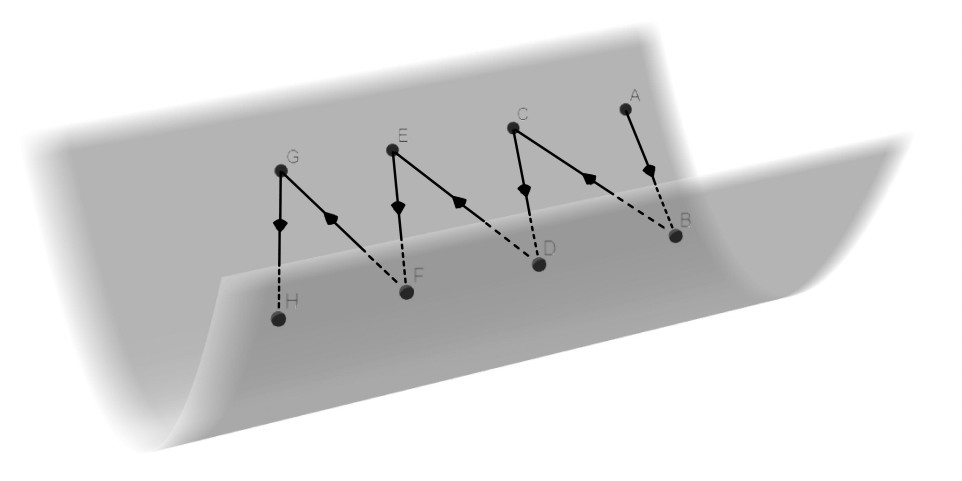
\includegraphics[width=0.7\linewidth]{pinched.png}
    \caption{A pinched landscape}
    \label{fig:pinched}
\end{figure}

As shown, gradient descent often `zigzags' along the alley rather than just moving down along it. 

\subsection*{Momentum Methods}

An easy fix for this is via the \textbf{momentum method}. To each iteration, we add a term proportional to the previous move, so that our iteration becomes
\[
    \mathbf{x}_{n+1} = \mathbf{x}_n - \alpha_n \cdot \nabla f(\mathbf{x}_n) + \beta_n (\mathbf{x}_n - \mathbf{x}_{n-1}).
\]
Usually, $\beta_n < \alpha_n$. For simplicity, we let $\alpha_n \equiv \alpha$ and $\beta_n \equiv \beta$. Setting $\mathbf{y}_n = \mathbf{x}_n - \mathbf{x}_{n-1}$, the iteration can be viewed of the following set of differential equations. 
\begin{align*}
    \dot{\mathbf{x}}(t) &= \mathbf{y}(t) \\
    \dot{\mathbf{y}}(t) &= -a \mathbf{y}(t) - \nabla f(\mathbf{x}(t))
\end{align*}
where $a \vcentcolon= (1 - \alpha/\beta) > 0$. This can be interpreted as Newtonian dynamics in a potential field $f$ with damping. A common example is a ball rolling down a rough hill. Thanks to its momentum, the ball is able to escape any points of local maxima, saddle points, inflection points, and even shallow local minima. It also does a better job of moving along a `flat' landscape than gradient descent. It quickly approaches the bottom of valleys where it eventually settles down, much faster than gradient dynamics. The iterate also locally oscillates dissipating energy before it settles down. 

\medskip 

Finally, note that we never evaluate the gradient analytically, but rather, it is approximated via one of the following schemes.
\begin{align*}
    \frac{\partial f}{\partial x_i}(\mathbf{x}) &\approx \frac{f(\mathbf{x} + \delta \mathbf{e}_i) - f(\mathbf{x})}{\delta} \\
    \frac{\partial f}{\partial x_i}(\mathbf{x}) &\approx \frac{f(\mathbf{x} + \delta \mathbf{e}_i) - f(\mathbf{x} - \delta \mathbf{e}_i)}{2\delta}
\end{align*}
The former requires only $d+1$ function evaluations while having a higher error of $\mathcal{O}(\delta)$. The latter requires $2d$ function evaluations but has a smaller error of $\mathcal{O}(\delta^2)$. 
\newpage
\section{Lecture 13}

\subsection*{Conjugate Gradient Method}

Let $f(\mathbf{x}) = \frac{1}{2} \mathbf{x}^{\top} \mathbf{Q} \mathbf{x} - \mathbf{b}^{\top} \mathbf{x}$ where $\mathbf{Q}$ is positive definite. This allows us to define an inner product
\[
    \left\langle \mathbf{x}, \mathbf{y} \right\rangle_{\mathbf{Q}} \vcentcolon= \mathbf{x}^{\top} \mathbf{Q} \mathbf{y}
\]
\begin{defn}[Conjugate Directions]
    $\{ \mathbf{d}_i \}_i \subseteq \mathbb{R}^d$ are said to be \emph{conjugate directions} if $\mathbf{d}_i \neq \mathbf{0}$ for all $i$, and
    \[
        \left\langle \mathbf{d}_i, \mathbf{d}_j \right\rangle_{\mathbf{Q}} = \mathbf{0} \quad \text{for all } i \neq j.
    \]
    Clearly, there are at most $d$ such conjugate directions.
\end{defn}

Now, consider the algorithm
\[
    \mathbf{x}_{n+1} = \mathbf{x}_n + \alpha_n \mathbf{d}_n
\]
where $\mathbf{d}_n$'s are chosen from the set of conjugate directions. Further, assume that exact line minimization is carried out. We then have
\[
    \alpha_n = \argmin_{\alpha} \, f(\mathbf{x}_n + \alpha \mathbf{d}_n) = \frac{\mathbf{d}_n^{\top} (\mathbf{b} - \mathbf{Qx}_n)}{\norm{\mathbf{d}_n}^2}
\]
Further, 
\[
    \nabla f(\mathbf{x}) = \mathbf{Qx} - \mathbf{b} \implies \nabla f(\mathbf{x}_n)^{\top} \mathbf{d}_i = 0 \quad \forall i < n.
\]
Thus, 
\[
    \mathbf{x}_{n+1} = \argmin_{\mathbf{x} \in \Span\{\mathbf{d}_i\}, 1 \leq i \leq n} f(\mathbf{x}).
\]
Thus, $\mathbf{x}_n$ converges to $\argmin f$ in at most $d$ steps. This is called the method of conjugate directions.

The conjugate gradient algorithm corresponds to the special case when the $\mathbf{d}_i$'s are computed by successively applying Gram-Schmidt orthogonalization to $-\nabla f(\mathbf{x}_n)$, $n \geq 0$, with respect to the inner product $\langle \cdot, \cdot \rangle_{\mathbf{Q}}$. Let $\mathbf{g}_n \vcentcolon= \nabla f(\mathbf{x}_n)$. Then, $\mathbf{g}_n \perp \mathbf{d}_i$ for $i < n$, so that $\mathbf{g}_n \perp \mathbf{g}_i$ for $i < n$. Further, we can easily show that
\[
    \mathbf{g}_n^{\top} \mathbf{Qd}_j = \begin{cases}
        0 & \text{for }0 \leq j < n-1, \text{ and} \\
        \displaystyle \frac{\mathbf{g}_n^{\top} \mathbf{g}_n}{\alpha_{n-1}} & \text{for } j = n-1.
    \end{cases}
\]
Furthermore, we have
\[
    \mathbf{d}_j^{\top} \mathbf{Qd}_j = \frac{1}{\alpha_j} \mathbf{d}_j^{\top} (\mathbf{g}_{j+1} - \mathbf{g}_j)
\]
Substituting this in the Gram-Schmidt formula, given by
\[
    \mathbf{d}_n = -\mathbf{g}_n + \sum_{j=0}^{n-1} \frac{\mathbf{g}_n^{\top} \mathbf{Qd}_j}{\mathbf{d}_j^{\top} \mathbf{Qd}_j} \cdot \mathbf{d}_j
\]
we get
\[
    \mathbf{d}_n = -\mathbf{g}_n + \beta_n \mathbf{d}_{n-1}
\]
where
\[
    \beta_n = \frac{\norm{\mathbf{g}_n}^2}{\mathbf{d}_{n-1}^{\top} (\mathbf{g}_n - \mathbf{g}_{n-1})}
\]

Simplifying this, we get the following conjugate gradient algorithm.

\begin{align*}
    \mathbf{x}_{n+1} &= \mathbf{x}_n + \alpha_n \mathbf{d}_n \\
    \mathbf{d}_{n+1} &= -\nabla f(\mathbf{x}_{n+1}) + \beta_{n+1} \mathbf{d}_n \\
    \alpha_n &= \frac{\mathbf{d}_n^{\top}(\mathbf{b} - \mathbf{Qx}_n)}{\mathbf{d}_n^{\top}\mathbf{Qd}_n} \\
    \beta_n &= \frac{\norm{\nabla f(\mathbf{x}_n)^2}}{\norm{\nabla f(\mathbf{x}_{n-1})}^2}
\end{align*}
The above choice of $\beta_n$ is called the \textbf{Fletcher-Reeves} formula. A better choice in practice is the \textbf{Polak-Ribiere} formula which generalizes to non-quadratic functions. This formula is as follows.

\[
    \beta_n = \frac{\left\langle \nabla f(\mathbf{x}_n), \nabla f(\mathbf{x}_n) - \nabla f(\mathbf{x}_{n-1}) \right\rangle}{\norm{\nabla f(\mathbf{x}_{n-1})}^2}
\]

\subsection*{Newton-Raphson Method}

Suppose you wish to solve for $f(\mathbf{x}) = \mathbf{0}$ for some $f \colon \mathbb{R}^d \to \mathbb{R}^d$. By virtue of Taylor expansion, we may write
\[
    f(\mathbf{x}_1) \approx f(\mathbf{x}_0) + \mathbf{D}f(\mathbf{x}_0) (\mathbf{x}_1 - \mathbf{x}_0).
\]
Assuming $f(\mathbf{x}_1) \approx \mathbf{0}$, we get
\begin{align*}
    \mathbf{x}_1 &= \mathbf{x}_0 + \mathbf{D}f(\mathbf{x}_0)^{-1} \left(f(\mathbf{x}_1) - f(\mathbf{x}_0) \right) \\
    &\approx \mathbf{x}_0 - \mathbf{D}f(\mathbf{x}_0)^{-1} f(\mathbf{x}_1).
\end{align*}

This gives us the iterative scheme
\[
    \mathbf{x}_{n+1} = \mathbf{x}_n - \alpha_n \mathbf{D}f(\mathbf{x}_n)^{-1} f(\mathbf{x}_n). 
\]
This scheme has been shown to work in practice most of the time. One can show that to ``minimize'' the error term at each iteration, one must use the following iterative scheme.
\[
    \mathbf{x}_{n+1} = \mathbf{x}_n - \alpha_n \left( \nabla^2 f(\mathbf{x}_n) \right)^{-1} \nabla f(\mathbf{x}_n).
\]
However, computing the Hessian at each step is extremely expensive. Furthermore, the estimation of the gradients and the Hessian poses several numerical issues such as the small divisor problem.  
\newpage
\section{Lecture 14}

Let $f(\mathbf{x}) \vcentcolon= \mathbf{Ax}$ where $\mathbf{A} \in \mathbb{R}^{m \times n}$ with $m \leq n$. 

\begin{thm}
    \begin{enumerate}
        \item If $\mathbf{A}$ is full rank, then for all $\mathbf{b} \in \mathbb{R}^m$, the set $\left\{ \mathbf{x} \in \mathbb{R}^n \colon \mathbf{Ax} = \mathbf{b} \right\}$ is an $(n-m)$ dimensional subspace of $\mathbb{R}^n$. 

        \item If $\mathbf{A}$ is not full rank, then the set $\mathcal{S} = \left\{ \mathbf{y} \in \mathbb{R}^m \colon \mathbf{Ax} = \mathbf{y} \right\}$ has dimension less than $n$. Moreover, the $m$-dimensional volume of $\mathcal{S}$ is $0$. 
    \end{enumerate}
\end{thm}

\begin{defn}[Manifold]
    A space $\mathcal{S}$ is a ($d$-dimensional) \emph{manifold} if it locally resembles Euclidean space at each point. More precisely, for every $\mathbf{x} \in \mathcal{S}$, there is an open neighbourhood $\mathcal{O}$ of $\mathbf{x}$ which can be invertibly mapped to $\mathbb{R}^d$. 
\end{defn}

Let $f \colon \mathcal{O} \to \mathbb{R}^d$ be the (invertible) map described above. $\mathcal{S}$ is a $\mathcal{C}^k$ manifold if $f,f^{-1}$ are $k$ times continuously differentiable. If $\mathcal{S}$ is a $\mathcal{C}^{\infty}$ manifold, then $\mathcal{S}$ is called a \emph{smooth} manifold and $f,f^{-1}$ are called \emph{diffeomorphisms}. If $f,f^{-1}$ are continuous, then $\mathcal{S}$ is called a \emph{topological} manifold and $f,f^{-1}$ are called \emph{homeomorphisms}.

\begin{thm}[Implicit Function Theorem]
    Let $\mathcal{S}$ be a $d$-dimensional smooth manifold and let $f \colon \mathcal{S} \to \mathbb{R}^k$ with $k < d$. If for some $\mathbf{x}_0 \in \mathcal{S}$ we have that $\mathbf{D}f(\mathbf{x}_0)$ is full rank (onto), then there exists an open neighbourhood $\mathcal{O}$ of $\mathbf{x}_0$ such that for $\mathbf{y} = f(\mathbf{x}_0)$, $\mathcal{O} \cap f^{-1}(\mathbf{y})$ is a \emph{unique} $(d-k)$ dimensional submanifold. 
\end{thm}

\begin{thm}[Sard's Theorem]
    Let $\mathcal{S}$ be a $d$-dimensional smooth manifold and let $f \colon \mathcal{S} \to \mathbb{R}^k$ with $k < d$. Let $X \subseteq \mathcal{S}$ denote the \emph{critical set} of $f$, that is, the set of points $\mathbf{x} \in \mathcal{S}$ such that $\mathbf{D}f(\mathbf{x})$ is not full-rank. Then, the image $f(X)$ has $k$-dimensional volume $0$. 
\end{thm}

The differential equation counterpart of the Newton scheme is
\[
    \Dot{\mathbf{x}}(t) = - \left( \nabla^2 f(\mathbf{x}(t)) \right)^{-1} \, \nabla f(\mathbf{x}(t)) =\vcentcolon \mathbf{h}(\mathbf{x}(t))
\]  
Let $E$ be the set of equilibria of the this equation, that is, $E = \left\{ \mathbf{x} \in \mathbb{R}^d \colon \mathbf{h}(\mathbf{x}) = \mathbf{0} \right\}$. Suppose that $E$ can be enclosed in a bounded region $D$ such that $\mathbf{h}$ is always pointing inwards at the boundary $\partial D$ of $D$. Now, away from $E$, $\norm{\nabla f(\mathbf{x})} > 0$ and we may define
\[
    \mathbf{g}(\mathbf{x}) \vcentcolon= \frac{\nabla f(\mathbf{x})}{\norm{\nabla f(\mathbf{x}}}.
\]
Further, $\mathbf{g}(\mathbf{x}) = \mathbf{c}$ represents a trajectory of the differential equation. Note that $\mathbf{g}$ maps $\mathbb{R}^d$ onto the unit $d$-sphere $\mathcal{S}_d \vcentcolon= \left\{ \mathbb{R}^d \colon \norm{\mathbf{x}} = 1 \right\}$ which is a $(d-1)$-dimensional object. Thus, we expect the inverse image of any $\mathbf{c} \in \mathcal{S}_d$ under $\mathbf{g}$ ($\mathbf{g}^{-1}(\mathbf{c})$) to be a $1$-dimensional curve in $\mathbb{R}^d$. If the conditions imposed in the Implicit Function Theorem hold, we may conclude by the Implicit Function Theorem that in a sufficiently small neighbourhood of any point in $D \setminus E$, there is a unique such curve. Starting from the boundary, we have the following. 
\begin{enumerate}
    \item The curve cannot intersect itself, 
    \item the curve cannot come arbitrarily close to itself, and
    \item the curve cannot end abruptly at a point in $D \setminus E$ since the Implicit Function Theorem allows us to extend it further.
    \item The curve cannot turn around and exit $D$ since $\mathbf{h}$ points inwards at $\partial D$.
\end{enumerate}
Thus, the curve must converge to $E$. Moreover, by Sard's Theorem, these arguments fail for $\mathbf{c}$ belonging to a set of measure zero. Thus, the Newton scheme works for `almost all' initial conditions.

\subsection*{Quasi-Newton Schemes}

Although the Newton scheme has a very reliable and sleek theory, it often runs into numerical issues in practice, since we can only estimate the gradients. This has led to the development of approximate methods known as \emph{quasi-Newton} methods. The idea is to keep track of a running recursive estimate of $\nabla^2 f(\mathbf{x}_n)^{-1}$ in a manner that ensures positive definiteness and the \emph{quasi-Newton} condition. We have
\[
    \nabla f(\mathbf{x}_{n+1}) - \nabla f(\mathbf{x}_n) \approx \nabla^2 f(\mathbf{x}_{n+1}) (\mathbf{x}_{n+1} - \mathbf{x}_n)
\]
Thus, the approximation $\mathbf{H}_{n+1}$ of $\nabla^2 f(\mathbf{x}_{n+1})^{-1}$ should satisfy the quasi-Newton condition
\[
    \mathbf{x}_{n+1} - \mathbf{x}_n = \mathbf{H}_{n+1} \left( \nabla f(\mathbf{x}_{n+1}) - \nabla f(\mathbf{x}_n) \right)
\]

A simple update scheme is to use a rank-1 update of the form $\mathbf{A} \mapsto \mathbf{A} + \mathbf{uu}^{\top}$ for a suitable $\mathbf{u}$. A lot of the early schemes used this update but faced numerical issues such as the small divisor problem. A more sophisticated approach is to a use rank-2 update of the form $\mathbf{A} \mapsto \mathbf{A} + \mathbf{uu}^{\top} + \mathbf{vv}^{\top}$ for suitable $\mathbf{u}, \mathbf{v}$. 

To this end, we introduce the notation 
\begin{align*}
    \mathbf{s}_n &\vcentcolon= \mathbf{x}_{n+1} - \mathbf{x}_n, \\
    \mathbf{y}_n &\vcentcolon= \nabla f(\mathbf{x}_{n+1}) - \nabla f(\mathbf{x}_n), \\
    \mathbf{w}_n &\vcentcolon= \frac{\mathbf{s}_n}{\mathbf{y}_n^{\top} \mathbf{s}_n} - \frac{\mathbf{H}_n \mathbf{y}_n}{\mathbf{y}_n^{\top} \mathbf{H}_n \mathbf{y}_n}.
\end{align*}

The quasi-Newton condition can then be written as
\[
    \mathbf{s}_n = \mathbf{H}_{n+1} \mathbf{y}_n.
\]
Now, we consider the rank-2 update
\[
    \mathbf{H}_{n+1} = \mathbf{H}_n + \alpha \mathbf{uu}^{\top} + \beta \mathbf{vv}^{\top}
\]
for suitable scalars $\alpha,\beta$ and vectors $\mathbf{u},\mathbf{v}$. By the quasi-Newton condition, we have
\[
    \mathbf{s}_n = \mathbf{H}_n\mathbf{y}_n + \alpha \mathbf{uu}^{\top} \mathbf{y}_n + \beta \mathbf{vv}^{\top} \mathbf{y}_n.
\]
We choose $\mathbf{u} = \mathbf{s}_n$, $\mathbf{v} = \mathbf{H}_n \mathbf{y}_n$, and $\alpha, \beta$ such that $\alpha \mathbf{u}^{\top} \mathbf{y}_n = 1$ and $\beta \mathbf{v}^{\top} \mathbf{y}_n = -1$. This leads to 
\[
    \mathbf{H}_{n+1} = \mathbf{H}_n + \frac{\mathbf{s}_n \mathbf{s}_n^{\top}}{\mathbf{s}_n^{\top} \mathbf{y}_n} - \frac{\mathbf{H}_n \mathbf{y}_n \mathbf{y}_n^{\top} \mathbf{H}_n}{\mathbf{y}_n^{\top} \mathbf{H}_n \mathbf{y}_n}.
\]
This is the original quasi-Newton scheme, now popularly known as the \textbf{Davidon-Fletcher-Powell} method. 

The general scheme is given by
\[
    \mathbf{x}_{n+1} = \mathbf{x}_n - \alpha_n \mathbf{H}_n \nabla f(\mathbf{x}_n)
\]
coupled with the iterates $\{ \mathbf{H}_n \}$ which are given by
\[
    \mathbf{H}_{n+1} = \mathbf{H}_n - \frac{\mathbf{H}_n \mathbf{y}_n \mathbf{y}_n^{\top}\mathbf{H}_n}{\mathbf{y}_n^{\top} \mathbf{H}_n \mathbf{y}_n} + \frac{\mathbf{s}_n \mathbf{s}_n^{\top}}{\mathbf{y}_n^{\top} \mathbf{s}_n} + \bm{\phi}_n \left( \mathbf{y}_n^{\top} \mathbf{H}_n \mathbf{y}_n \right) \mathbf{w}_n \mathbf{w}_n^{\top}. 
\]
This family of algorithms is known as the \textbf{Broyden} family. Here, $\bm{\phi}_n \in [0,1]$ is a flexible parameter which can be chosen based on $\mathbf{y}_n, \mathbf{s}_n,$ and $\mathbf{w}_n$. The choice of $\bm{\phi}_n \equiv 0$ gives us the Davidon-Fletcher-Powell method. The choice $\bm{\phi}_n \equiv 1$ gives us the \textbf{Broyden-Fletcher-Goldfarb-Shanno} (\textbf{BFGS}) algorithm. 

Note that $\mathbf{w}_n \perp \mathbf{y}_n$. Thus, any quantity proportional to $\mathbf{w}_n\mathbf{w}_n^{\top}$ can be added on the right hand side without affecting $\mathbf{s}_n$. The last term does however affect the convergence behaviour of the algorithm and gives practitioners and additional handle to tweak. 
\newpage
\section{Lecture 15}

We now prove the correctness of the quasi-Newton scheme. Suppose $\mathbf{H}_n$ is positive definite and $\alpha_n$ is chosen so that for $\mathbf{d}_n \vcentcolon= -\mathbf{H}_n \nabla f(\mathbf{x}_n)$, we have
\[
    \left\langle \nabla f(\mathbf{x}_n), \mathbf{d}_n \right\rangle < \left\langle \nabla f(\mathbf{x}_{n+1}), \mathbf{d}_n \right\rangle.
\]
This ensures that $\mathbf{H}_{n+1}$ is positive definite. If $\nabla f(\mathbf{x}_n) \neq \mathbf{0}$, then the above can be ensured by doing a line search till
\[
    \abs{\left\langle \nabla f(\mathbf{x}_n), \mathbf{d}_n \right\rangle} > \abs{\left\langle \nabla f(\mathbf{x}_{n+1}), \mathbf{d}_n \right\rangle}
\]
for example, by line minimization for which the right hand side is in fact zero. Then, $\alpha_n > 0$, $\mathbf{y}_n \neq \mathbf{0}$, and
\[
    \mathbf{s}_n^{\top} \mathbf{y}_n = \alpha_n \mathbf{d}_n^{\top} \left( \nabla f(\mathbf{x}_{n+1}) - \nabla f(\mathbf{x}_n) \right) > 0,
\]
so that all the denominators in the Broyden family are non-zero and $\mathbf{H}_{n+1}$ is well-defined. For $\mathbf{z} \neq \mathbf{0}$, let $\mathbf{a} \vcentcolon= \sqrt{\mathbf{H}_n} \mathbf{z}$, and let $\mathbf{b} \vcentcolon= \sqrt{\mathbf{H}_n} \mathbf{y}_n$. Then, 
\begin{align*}
    \mathbf{z}^{\top} \mathbf{H}_{n+1} \mathbf{z} &= \mathbf{z}^{\top}\mathbf{H}_n \mathbf{z} + \frac{\left(\mathbf{z}^{\top} \mathbf{s}_n\right)^2}{\mathbf{y}_n^{\top} \mathbf{s}_n} - \frac{\left( \mathbf{y}_n^{\top} \mathbf{H}_n \mathbf{z} \right)^2}{\mathbf{y}_n^{\top}\mathbf{H}_n\mathbf{y}_n} + \bm{\phi}_n \left( \mathbf{y}_n^{\top}\mathbf{H}_n\mathbf{y}_n \right) \left( \mathbf{w}_n^{\top} \mathbf{z} \right)^2 \\
    &= \frac{\norm{\mathbf{a}}^2 \norm{\mathbf{b}}^2 - \left( \mathbf{a}^{\top}\mathbf{b} \right)^2}{\norm{\mathbf{b}}^2} + \frac{\left(\mathbf{z}^{\top} \mathbf{s}_n\right)^2}{\mathbf{y}_n^{\top} \mathbf{s}_n} + \bm{\phi}_n \left( \mathbf{y}_n^{\top}\mathbf{H}_n\mathbf{y}_n \right) \left( \mathbf{w}_n^{\top} \mathbf{z} \right)^2.
\end{align*}
We leave it as an exercise to show that this is in fact positive, which proves the positive definiteness of $\mathbf{H}_{n+1}$. 

A `dual' scheme for updating the Hessians $\nabla^2 f(\mathbf{x}_n)$ rather than the inverse Hessian $(\nabla^2 f(\mathbf{x}_n))^{-1}$ can also be derived with $\mathbf{s}_n$ and $\mathbf{y}_n$ interchanged. This, however, requires matrix inversion which takes $\mathcal{O}(d^3)$ time. The current scheme can be reduced to $\mathcal{O}(d^2)$ using Cholesky decomposition. On the other hand, the dual scheme handles numerical errors better avoiding loss of positive definiteness better than the current scheme. 

A related scheme is the \textbf{Gauss-Newton} method which minimizes the square of the linear approximation
\[
    f(\mathbf{x}) \approx f(\mathbf{x}_n) + \left\langle \nabla f(\mathbf{x}_n), \mathbf{x} - \mathbf{x}_n \right\rangle. 
\]
This, in principle, leads to
\[
    \mathbf{x}_{n+1} = \mathbf{x}_n - \alpha_n \left( \nabla f(\mathbf{x}_n) \nabla f(\mathbf{x}_n)^{\top} \right)^{-1} \nabla f(\mathbf{x}_n) f(\mathbf{x}_n). 
\]
However, the rank-1 matrix $\nabla f(\mathbf{x}_n) \nabla f(\mathbf{x}_n)^{\top}$ is not invertible. Thus, we instead use the scheme
\[
    \mathbf{x}_{n+1} = \mathbf{x}_n - \alpha_n \left( \nabla f(\mathbf{x}_n) \nabla f(\mathbf{x}_n)^{\top} + \bm{\Delta} \right)^{-1} \nabla f(\mathbf{x}_n) f(\mathbf{x}_n)
\]
where $\bm{\Delta}$ is a small positive definite matrix. The choice $\bm{\Delta} = \nu \mathbf{I}$ leads to the \textbf{Levenberg-Marquadt} method, which is extremely popular in neural networks literature. 
\newpage
\section{Lecture 16}

Here we consider solution schemes for the generalized \textbf{constrained optimization} problem, defined as 
\begin{equation}
    \label{constrained}
    \text{Minimize } f(\mathbf{x}) \text{ on } C \vcentcolon= \left\{ \mathbf{x} \colon g_i(\mathbf{x}) \leq 0 \quad 1 \leq i \leq M \right\} \tag{P}
\end{equation}

\subsection*{Penalty Functions}

Instead of solving \eqref{constrained}, one minimizes, without constrains, the function $f_{\lambda}(\mathbf{x}) \vcentcolon= f(\mathbf{x}) + \lambda F(\mathbf{x})$ where the \textit{penalty function} $F(\mathbf{x})$ is chosen such that as $\lambda \to \infty$, $\lambda F(\mathbf{x}) \to 0$ on $C$, and $\to \infty$ on $C^{\mathsf{c}}$ uniformly on closed bounded sets. Thus, if $\mathbf{x}^*(\lambda)$ is a minimizer of $f_{\lambda}$ then any limit point of $\mathbf{x}^*(\lambda)$ as $\lambda \uparrow \infty$ should be a solution to \eqref{constrained}. The solution to this \textit{unconstrained} problem thus approximates the solution of the original constrained problem. Typically, the optimal solution to \eqref{constrained} is on the boundary $\partial C$ but $\mathbf{x}^*(\lambda) \notin C$. Thus, $\mathbf{x}^*(\lambda)$ is not feasible and one generally takes the point closest to it in $C$ as an approximate solution. Usually, one choses $F$ to be continuously differentiable such that there is at least one minimizer of $f_{\lambda}$. A popular choice is
\[
    F(\mathbf{x}) \vcentcolon= \sum_{i=1}^M \left( g_i^+(\mathbf{x}) \right)^2.
\]

\subsection*{Barrier Functions}

The penalty function method approximates the solution to \eqref{constrained} from `the outside'. Barrier function methods follow the same philosophy but approximate the solution to \eqref{constrained} from `the inside', that is, from the interior of $C$ (recall that this is denoted as $\interior{C}$). The idea is to minimize $f_{\mu}(\mathbf{x}) \vcentcolon= f(\mathbf{x}) + \mu F(\mathbf{x})$ on $\interior{C}$ with a \textit{barrier function} $F \colon \interior{C} \to \mathbb{R}$ satisfying $F(\mathbf{x}) \to \infty$ as $\mathbf{x} \to \partial C$ and $f_{\mu} \to f$ on $\interior{C}$ as $\mu \downarrow 0$. One popular example is the logarithmic barrier:
\[
    F(\mathbf{x}) \vcentcolon= \sum_{i=1}^M \log \left( - \frac{1}{g_i(\mathbf{x})} \right).
\]

Barrier function methods form an important class of interior point methods used in convex optimization. 

\subsection*{Primal-Dual Methods}

These schemes are based on the Lagrange multiplier rule, the idea being to find the saddle point in $(\mathbf{x}, \bm{\Lambda})$ of $f(\mathbf{x}) + \bm{\Lambda}^{\top} g(\mathbf{x})$. One such method is the \textbf{gradient ascent-descent} scheme that uses the coupled iteration:
\begin{align*}
    \mathbf{x}_{n+1} &= \mathbf{x}_n - \alpha_n \left( \nabla f(\mathbf{x}_n) + \sum_{i=1}^M \Lambda_{n,i} \nabla g_i(\mathbf{x}_n) \right) \\
    \bm{\Lambda}_{n+1} &= \left[ \bm{\Lambda}_n + \alpha_n g(\mathbf{x}_n) \right]^+
\end{align*}
where $[ \,\cdot\, ]^+$ is applied component-wise. The differential equation counterpart is
\begin{align*}
    \Dot{\mathbf{x}}(t) &= - \nabla \left( f + \bm{\Lambda}(t)^{\top} g \right) (\mathbf{x}(t)), \\
    \Dot{\bm{\Lambda}}(t) &= g(\mathbf{x}(t)). 
\end{align*}
constrained to remain in $\mathbb{R}^d \times \mathbb{R}^M_+$. For strictly convex $f,g$, let $(\mathbf{x}^*, \bm{\Lambda}^*)$ be the (unique) saddle point. Then, 
\[
    V(\mathbf{x}, \bm{\Lambda}) \vcentcolon= \frac{1}{2} \norm{\mathbf{x} - \mathbf{x}^*}^2 + \frac{1}{2} \norm{\bm{\Lambda} - \bm{\Lambda}^*}^2
\]
serves as a Lyapunov function. 

\subsection*{Projected Gradient}

Consider the hyperplane $\mathcal{H} \vcentcolon= \left\{ \mathbf{x} \in \mathbb{R}^d \colon \mathbf{Ax} = \mathbf{0}\right\}$. The projection of $\mathbf{x} \in \mathbb{R}^d$ onto $\mathcal{H}$ is given by
\[
    \Gamma (\mathbf{x}) \vcentcolon= \left( \mathbf{I} - \mathbf{A}^{\top} (\mathbf{AA}^{\top})^{-1} \mathbf{A} \right) \mathbf{x}. 
\]
Then, $\Gamma(\cdot)$ satisfies the following. 
\begin{enumerate}
    \item $\norm{\Gamma(\mathbf{x}) - \mathbf{x}} \leq \norm{\mathbf{y} - \mathbf{x}}$ for all $\mathbf{y} \in \mathcal{H}$.
    \item $\Gamma(\mathbf{x}) = \mathbf{x}$ for all $\mathbf{x} \in \mathcal{H}$.
    \item $\Gamma$ is idempotent. That is, $\Gamma \circ \Gamma = \Gamma$.
\end{enumerate}

A general idea of the algorithm is that we start with unconstrained minimization. The moment we step out of the feasible region, we ``pull'' the iterate back into the feasible region. Suppose $h(\mathbf{x}) = \mathbf{0}$ denotes the active constraints. Then, $\left\{ \mathbf{y} \colon \mathbf{x} + Dh(\mathbf{x}) (\mathbf{y} - \mathbf{x}) = \mathbf{0} \right\}$ is the tangent plane at $\mathbf{x}$. The iterative scheme proceeds by taking the projection of the gradient onto the constraint set. That is,
\[
   \mathbf{x}_{n+1} = \bm{\Phi} \left( \mathbf{x}_n - \alpha_n \left( \mathbf{I} - \mathbf{A}^{\top} (\mathbf{AA}^{\top})^{-1} \mathbf{A} \right) \nabla f(\mathbf{x}_n) \right) 
\]
where $\mathbf{A} = Dh(\mathbf{x}_n)$ and $\bm{\Phi}$ is a suitable map to pull the iterate back to the feasible region, given by $\bm{\Phi}(\mathbf{y}) \vcentcolon= \mathbf{y} + Dh(\mathbf{x}_n)^{\top} \bm{\alpha}$ such that $h(\bm{\Phi}(\mathbf{y})) = \mathbf{0}$. $\bm{\alpha}$ can be found by Newton-Raphson. 

\subsection*{Reduced Gradient}

This method belongs to a class of algorithms called \textit{feasible direction methods}. At each step, the algorithm seeks to find an update direction such that the resulting solution is adjudged beforehand to be feasible. This is in contrast to the projected gradient method where we first perform unconstrained minimization and then project the solution back to the feasible set. 

Suppose we have linear constraints of the form $\mathbf{Ax} = \mathbf{b}$ where $\mathbf{A} = \begin{bmatrix} \mathbf{B} & \mathbf{C} \end{bmatrix}$ for some square non-singular matrix $\mathbf{B}$. Writing $\mathbf{x} = (\mathbf{y}, \mathbf{z})$ we may treat $\mathbf{z}$ as the independent variables and $\mathbf{y} = \mathbf{B}^{-1}(\mathbf{b} - \mathbf{Cz})$ as the dependent variables. We may then write
\begin{align*}
    \nabla f(\mathbf{y}, \mathbf{z}) &= \nabla f\left( \mathbf{B}^{-1}(\mathbf{b} - \mathbf{Cz}), \mathbf{z} \right) \\
    &= \nabla^{\mathbf{z}} f(\mathbf{y}, \mathbf{z}) - \nabla^{\mathbf{y}} f(\mathbf{y}, \mathbf{z}) \mathbf{B}^{-1}\mathbf{C}. 
\end{align*}

This prompts us to use the following scheme. Write $\mathbf{x}_n = (\mathbf{y}_n, \mathbf{z}_n)$ where $\mathbf{y}_n, \mathbf{z}_n$ are the dependent and independent parts respectively. Let $D^{\mathbf{r}}$ denote the Jacobian matrix w.r.t variables $\mathbf{r}$. Then, we let
\begin{align*}
    \mathbf{z}_{n+1} &= \mathbf{z}_n - \alpha_n \left( \nabla^{\mathbf{z}} f(\mathbf{y}_n, \mathbf{z}_n) - \nabla^{\mathbf{y}} f(\mathbf{y}_n, \mathbf{z}_n) \underbrace{D^{\mathbf{y}} h(\mathbf{y}_n, \mathbf{z}_n)^{-1}}_{\mathbf{B}^{-1}} \underbrace{D^{\mathbf{z}} h(\mathbf{y}_n, \mathbf{z}_n)}_{\mathbf{C}}  \right), \\
    \mathbf{y}_{n+1} &= \mathbf{y}_n - D^{\mathbf{y}} h(\mathbf{y}_n, \mathbf{z}_n)^{-1} D^{\mathbf{z}} h(\mathbf{y}_n, \mathbf{z}_n) \left( \mathbf{z}_{n+1} - \mathbf{z}_n \right).
\end{align*}

Note: In theory, we do not need to pull the iterate back into the feasible region. However, due to discretization errors, which are not intrinsic to the algorithm, we employ a similar Newton iteration to pull the iterate back to the feasible set.  
\newpage
\section{Lecture 17}

\subsection*{Conditional Gradient or Frank-Wolfe Method}

This is another popular feasible directions method. Here, we wish to minimize $f$ over a closed bounded feasible set $C$. At the $(n+1)^{\text{th}}$ iteration, we compute the direction $\mathbf{d}_n$ that is maximally aligned with $-\nabla f(\mathbf{x}_n)$ subject to the given constraints. That is,
\[
    \mathbf{d}_n \vcentcolon= \argmin_{\mathbf{z} \in C} \left\langle \nabla f(\mathbf{x}_n), \mathbf{z} \right\rangle.
\]  
The iterate is then given by
\[
    \mathbf{x}_{n+1} = (1-\alpha_n) \mathbf{x}_n + \alpha_n \mathbf{d}_n. 
\]
We choose $\alpha_n \in (0,1)$ such that $\sum_n \alpha_n = \infty$. Also, note that $\mathbf{x}_n \in C \implies \mathbf{x}_{n+1} \in C$ by convexity. 

\subsection*{Cutting Plane Method}

Consider convex $f,g$. It suffices to consider a linear objective $f(\mathbf{x}) = \mathbf{c}^{\top}\mathbf{x}$, since we can equivalently consider the problem of minimizing $r \in \mathbb{R}$ subject to $f(\mathbf{x}) - r \leq 0$, $g(\mathbf{x}) \leq \mathbf{0}$. Suppose the minimum is attained. Start with an initial polytope $P_1$ containing $C$. At step $n$, given a polytope $P_n$ containing $C$, do the following:
\begin{enumerate}
    \item Find $\mathbf{w}_n \vcentcolon= \argmin_{P_n} \mathbf{c}^{\top} \mathbf{x}$. If $g(\mathbf{w}_n) \leq \mathbf{0}$, stop. If not, go to step 2.
    \item Let $i^*_n \vcentcolon= \argmax_i g_i(\mathbf{w}_n)$. Then, $g_{i^*_n}(\mathbf{w}_n) > 0$. Set
    \[
        P_{n+1} = P_n \cup \left\{ \mathbf{x} \colon g_{i^*_n}(\mathbf{w}_n) + \left\langle \nabla g_{i^*_n}(\mathbf{w}_n), \mathbf{x} - \mathbf{w}_n \right\rangle \leq 0. \right\}
    \]
    Repeat till convergence. 
\end{enumerate}

It is easy to see that $\mathbf{w}_n \notin P_{n+1}$. Thus, the next polytope excludes the current minimizer. Also, for $\mathbf{x} \in C$, 
\[
    0 \geq g_{i^*_n}(\mathbf{x}) \geq g_{i^*_n}(\mathbf{w}_n) + \left\langle \nabla g_{i^*_n}(\mathbf{w}_n), \mathbf{x} - \mathbf{w}_n \right\rangle
\]
which implies that $C \subseteq P_{n+1}$. Thus, the next polytope retains the entire constraint set. 

Now, suppose that $\mathbf{w}_{n_k} \to \mathbf{w}^*$ where $n_k$ are such that $i^*_{n_k} \equiv \hat{i}$ (say). Since there are only finite many indices, such a subsequence must exist. Moreover, convergence follows by Bolzano-Weierstrass. Then, we have
\[
    \nabla g_{\hat{i}}(\mathbf{w}_{n_k}) \to \nabla g_{\hat{i}}(\mathbf{w}^*)
\]
implying $\sup_k \norm{\nabla g_{\hat{i}}(\mathbf{w}_{n_k})} < \infty$. Then, 
\begin{align*}
    g_{\hat{i}}\left( \mathbf{w}_{n+m} \right) &\leq \left\langle -\nabla g_{\hat{i}}(\mathbf{w}_{n_k}),   \mathbf{w}_{n+m} - \mathbf{w}_n \right\rangle \\
    &\leq \norm{\nabla g_{\hat{i}}(\mathbf{w}_{n_k})} \norm{\mathbf{w}_{n+m} - \mathbf{w}_n} \\
    \implies g_{\hat{i}}(\mathbf{w}^*) &\leq 0 \quad (\text{on letting } k \uparrow \infty) \\
    \implies g_i(\mathbf{w}^*) &\leq 0 \quad \forall i. 
\end{align*}

Thus, $\mathbf{w}^*$ is feasible. Optimality follows by a limiting argument. 

\subsection*{Two Timescale Schemes}

This is the coupled iteration
\begin{align*}
    \mathbf{x}_{n+1} &= \mathbf{x}_n + \alpha_n h(\mathbf{x}_n, \mathbf{y}_n), \\
    \mathbf{y}_{n+1} &= \mathbf{y}_n + \beta_n g(\mathbf{x}_n, \mathbf{y}_n).
\end{align*}
Here $h,g$ are assumed to be Lipschitz and $\alpha_n, \beta_n > 0$ satisfy $\sum_n \alpha_n = \sum_n \beta_n = \infty$, and $\beta_n = o(\alpha_n)$. The latter condition ensures that the second iteration moves at a slower time scale than the first one, and is approximately constant (to be precise, very slowly-varying) on the timescale of the first iteration. Thus, the first iteration tracks the ODE
\[
    \Dot{\mathbf{x}}^{\prime}(t) = h( \mathbf{x}^{\prime}(t), \mathbf{y})
\]
for $\mathbf{y} \approx \mathbf{y}(t)$. Suppose this $\mathbf{x}^{\prime}(t)$ converges to a unique $\Lambda(\mathbf{y})$ where $\Lambda(\cdot)$ is Lipschitz. This implies that $\mathbf{x}_n - \Lambda(\mathbf{y}_n) \to 0$ asymptotically. Thus, the second iteration tracks the ODE
\[
    \Dot{\mathbf{y}}^{\prime}(t) = g\left( \Lambda(\mathbf{y}^{\prime}(t)), \mathbf{y}^{\prime}(t) \right).
\]
Suppose this converges to some $\mathbf{y}^*$. Then, the coupled iterate converges to $(\Lambda(\mathbf{y}^*), \mathbf{y}^*)$. Thus, $\{\mathbf{x}_n\}$ sees $\{\mathbf{y}_n\}$ as quasi-static, and $\{\mathbf{y}_n\}$ sees $\{\mathbf{x}_n\}$ as quasi-equilibriated. Two timescale schemes are frequently used to replace a subroutine on a concurrent iteration. One example is the use of two timescales in actor-critic methods in reinforcement learning.

\subsection*{Homotopy Methods}

Let $f,g \colon \mathbb{R}^d \to \mathbb{R}$. $f$ is said to be \textit{homotopic} to $g$ if there exists a continuous deformation $F \colon \mathbb{R}^d \times [0,1] \to \mathbb{R}$ such that 
\[
    F(\mathbf{x},0) = g(\mathbf{x}), F(\mathbf{x},1) = f(\mathbf{x}) \quad \text{for all } \mathbf{x} \in \mathbb{R}^d. 
\]
A standard example is the map
\[
    F(\mathbf{x},t) = (1-t) g(\mathbf{x}) + t f(\mathbf{x}).
\]
To find the minimizer of $f$, you start with a strictly convex curve $g$ and slowly deform it to $f$. Let $\mathbf{x}_0$ be the minimizer of $g$. We track the solution $\mathbf{x}^*(t), t \in [0,1]$ of $\nabla_{\mathbf{x}} F(\mathbf{x},t) = \mathbf{0}$ with the initial condition $\mathbf{x}^*(0) = \mathbf{x}_0$, as $t \to 1$. This gives us the two timescale iteration
\begin{align*}
    \mathbf{x}_{n+1} &= \mathbf{x}_n - \alpha_n \left( \nabla_{\mathbf{x}}^2 F(\mathbf{x}_n, t_n) \right)^{-1} \nabla_{\mathbf{x}} F(\mathbf{x}_n, t_n), \\
    t_{n+1} &= t_n + \beta_n \quad (\text{slowly increase to } 1). 
\end{align*}
This guarantees a continuous curve to a critical point of $f$ using a parametric form of Sard's Theorem. 
\newpage
\section{Lecture 18}

\subsection*{Convex-Concave Procedure}

This is sometimes also known as `Difference of Convex' (DC) programming. Let $f \colon \mathbb{R}^d \to \mathbb{R}$ be twice continuously differentiable such that the eigenvalues of $\nabla^2 f(\mathbf{x})$ are bounded in absolute value by some $K < \infty$ for all $\mathbf{x}$. Then, we may write 
\[
    f(\mathbf{x}) = \left( f(\mathbf{x}) + K\norm{\mathbf{x}}^2 \right) + \left( - K\norm{\mathbf{x}}^2 \right)
\]
as a sum of a convex and a concave function. More generally, consider the problem of minimizing $f = h + g$ where $h,g$ are continuously differentiable, $h$ is convex, and $g$ is concave. The convex-concave procedure solves
\[
    \nabla h(\mathbf{x}_{n+1}) = -\nabla g(\mathbf{x}_n)
\]
to get $\mathbf{x}_{n+1}$ from $\mathbf{x}_n$. By convexity, one has
\begin{align*}
    h(\mathbf{x}_n) &\geq h(\mathbf{x}_{n+1}) + \left\langle \nabla h(\mathbf{x}_{n+1}) , \mathbf{x}_n - \mathbf{x}_{n+1} \right\rangle \\
    \implies h(\mathbf{x}_{n+1}) &\leq h(\mathbf{x}_n) - \left\langle \nabla h(\mathbf{x}_{n+1}) , \mathbf{x}_n - \mathbf{x}_{n+1} \right\rangle \\
    &= h(\mathbf{x}_{n+1}) \leq h(\mathbf{x}_n) + \left\langle \nabla g(\mathbf{x}_n) , \mathbf{x}_n - \mathbf{x}_{n+1} \right\rangle \\
    &= h(\mathbf{x}_{n+1}) \leq h(\mathbf{x}_n) - \left\langle \nabla g(\mathbf{x}_n) , \mathbf{x}_{n+1} - \mathbf{x}_n \right\rangle.
\end{align*}
Likewise by concavity, we get
\[
    g(\mathbf{x}_{n+1}) \leq g(\mathbf{x}_n) + \left\langle \nabla g(\mathbf{x}_n) , \mathbf{x}_{n+1} - \mathbf{x}_n \right\rangle.
\]
Adding the two, we get
\[
    f(\mathbf{x}_{n+1}) \leq f(\mathbf{x}_n). 
\]
Thus, this scheme guarantees monotone behaviour and the procedure thus stops at a minima. 

\subsection*{Proximal Methods}

Define the \textit{proximal} operator as
\[
    \prox_{\lambda f}(\mathbf{u}) \vcentcolon= \argmin_{\mathbf{x}} \left( f(\mathbf{x}) + \frac{1}{2\lambda} \norm{\mathbf{x} - \mathbf{u}}^2 \right).
\]
The proximal algorithm performs the following iteration.
\[
    \mathbf{x}_{n+1} = \prox_{\alpha_n f}(\mathbf{x}_n) = \argmin_{\mathbf{x}} \left( f(\mathbf{x}_n) + \frac{1}{2\alpha_n} \norm{\mathbf{x} - \mathbf{x}_n}^2 \right).
\]
By adding a quadratic penalty, one ensures that $\mathbf{x}_{n+1}$ does not move too far away from $\mathbf{x}_n$. The minimum condition at each iteration yields the following.
\[
    \mathbf{0} \in \partial \left( f(\cdot) + \frac{1}{2\alpha_n} \norm{\cdot - \mathbf{x}_n}^2 \right) \rvert_{\mathbf{x}_{n+1}} = \partial f(\mathbf{x}_{n+1}) + \frac{1}{\alpha_n} \left( \mathbf{x}_{n+1} - \mathbf{x}_n \right).
\] 
Thus, 
\[
    \mathbf{x}_{n+1} \in \mathbf{x}_n - \alpha_n \partial f(\mathbf{x}_{n+1}). 
\]
Where $\partial f$ denotes a subgradient of $f$. If the subgradient is in fact a gradient, then the above corresponds to the `backward Euler scheme' for solving 
\[
    \Dot{\mathbf{x}}(t) = -\nabla f(\mathbf{x}(t)).
\]

Let
\[
    \bm{\Psi}_f(\mathbf{u}) \vcentcolon= \inf_{\mathbf{x}} \left( f(\mathbf{x}_n) + \frac{1}{2} \norm{\mathbf{x} - \mathbf{u}}^2 \right).
\]
By the definition of the proximal operator, 
\[
    \bm{\Psi}_{\lambda f}(\mathbf{x}) = f\left( \prox_{\lambda f}(\mathbf{x}) \right) + \frac{1}{2\lambda} \norm{\mathbf{x} - \prox_{\lambda f}(\mathbf{x})}^2.
\]
By Danskin's theorem, we have
\[
    \nabla \bm{\Psi}_{\alpha_n f} (\mathbf{x}_n) = \frac{\mathbf{x}_{n+1} - \mathbf{x}_n}{\alpha_n}.
\]
That is,
\[
    \mathbf{x}_{n+1} = \mathbf{x}_n - \alpha_n \nabla \bm{\Psi}_{\alpha_n f} (\mathbf{x}_n)
\]
which is an explicit formulation. 

\subsection*{Proximal Gradient Method}

The \textit{proximal gradient} method deals with the minimization of functions of the form $\mathbf{x} \in \mathbb{R}^d \mapsto f(\mathbf{x}) + g(\mathbf{x})$ where $f \colon \mathbb{R}^d \to \mathbb{R}$ and $g \colon \mathbb{R}^d \to \mathbb{R} \cup \{\infty\}$. We further assume that $f$ is differentiable and that $\lim_{\norm{\mathbf{x}} \uparrow \infty} f(\mathbf{x}) = \lim_{\norm{\mathbf{x}} \uparrow \infty} g(\mathbf{x}) = \infty$. The algorithm is given by
\[
    \mathbf{x}_{n+1} = \prox_{\alpha_n g} \left( \mathbf{x}_n - \alpha_n \nabla f(\mathbf{x}_n) \right).
\]  
Since $g$ is allowed to take value $\infty$, we can impose the convex constraint $\mathbf{x} \in C$ for a closed convex set $C$ by taking $g(\mathbf{x}) = 0$ for $\mathbf{x} \in C$ and $g(\mathbf{x}) = \infty$ for $\mathbf{x} \notin C$. 

This scheme again faces problems with `pinched' landscapes. We can modify the definition of the proximal operator by replacing the term $\frac{1}{2} \norm{\mathbf{x} - \mathbf{y}}^2$ by a more general distance measure $D(\mathbf{x}; \mathbf{y})$. A popular choice is the \textbf{Bregman divergence}
\[
    f(\mathbf{y}) - f(\mathbf{x}) - \left\langle \nabla f(\mathbf{x}), \mathbf{y} - \mathbf{x} \right\rangle \approx \frac{1}{2} (\mathbf{y} - \mathbf{x})^{\top} \nabla^2 f(\mathbf{x}) (\mathbf{y} - \mathbf{x})
\]
which leads to the popular \textbf{mirror descent algorithm}.

\subsection*{Separable Problems}

Consider minimizing $\sum_{i=1}^n f_i(x_i)$ subject to $\sum_{i} g(x_i) \leq 0$. If the Lagrange multiplier $\bm{\Lambda}$ is known, this splits into separable problems: minimize $f_i(x_i) + \bm{\Lambda}^{\top} g_i(x_i)$ for each $i$. This suggests the dual ascent scheme:
\begin{align*}
    x_{i,n} &= \argmin \left( f(\cdot) + \bm{\Lambda}_n^{\top} g_i(\cdot) \right) \quad \forall i, \\
    \bm{\Lambda}_{n+1} &= \bm{\Lambda}_n + \alpha_n \left( \sum_i g_i(x_{i,n}) \right).
\end{align*}
\end{document}